\chapter{การฝึกที่มีประสิทธิภาพและคำแนะนำเพิ่มเติม}
\label{chapter: Suggestions for ANN}

\begin{verse}
``Failure is the key to success;
each mistake teaches us something.''
--- Morihei Ueshiba
\end{verse}

\begin{verse}
``ความล้มเหลวคือกุญแจสู่ความสำเร็จ
แต่ละความผิดพลาดสอนเราบางอย่าง''
--- โมริเฮอิ อุเอชิบะ
\end{verse}

บทที่~\ref{chapter: ANN} อธิบายทฤษฎีพื้นฐานของโครงข่ายประสาทเทียม.
บทที่~\ref{chapter: Applications of ANN} แสดงตัวอย่างการประยุกต์ใช้โครงข่ายประสาทเทียม.
บทนี้จะถกถึงการฝึกที่มีประสิทธิภาพมากขึ้น และคำแนะนำสำหรับการประยุกต์ใช้โครงข่ายประสาทเทียม.

โครงข่ายประสาทเทียมที่ฝึกเสร็จแล้วจะสามารถทำการคำนวณได้อย่างรวดเร็ว.
แต่หากผู้อ่านได้ทดลองทำตามตัวอย่างในบทที่~\ref{chapter: Applications of ANN} คงพอรู้สึกว่า การเตรียมและการฝึกโครงข่ายประสาทเทียมจะใช้เวลาพอสมควร.
\textit{เวลาที่ใช้ในการฝึก}ก็ขึ้นอยู่กับ\textit{ขนาดข้อมูลฝึก} \textit{ขนาดของโครงข่าย} 
และ\textit{พารามิเตอร์ของการฝึก}.
ข้อมูลฝึกที่มีหลายมิติก็เท่ากับบังคับให้\textit{ตัวแปรค่าน้ำหนัก}มีขนาดใหญ่ขึ้น (สมการ~\ref{eq: ANN 2-layer z}, ค่าน้ำหนักของโครงข่ายชั้นที่หนึ่ง $\mathbf{W}^{(1)} \in \mathbb{R}^{M \times (1+D)}$ 
%เมื่อ $M$ แทนจำนวนหน่วยซ่อนของโครงข่ายประสาทเทียม และ 
โดย $D$ แทนจำนวนมิติของอินพุต)
ข้อมูลมีจำนวนจุดข้อมูลมาก ก็ทำให้แต่ละรอบฝึกต้องคำนวณกับข้อมูลมากขึ้น
โครงข่ายประสาทเทียมที่มีขนาดใหญ่ก็มีจำนวนค่าน้ำหนักที่ต้องคำนวณมากขึ้น
จำนวนรอบฝึกมากขึ้นก็จะใช้เวลาฝึกนานขึ้น.

อย่างที่ถกกันไป การฝึกโครงข่ายประสาทเทียมจริงๆแล้วก็คือ\textit{การหาค่าตัวทำน้อยที่สุด} โดย\textit{ตัวทำน้อยที่สุด}ที่ต้องการหาก็คือ\textit{ค่าน้ำหนัก} 
และ\textit{ฟังชั่นจุดประสงค์}ที่ต้องการให้มีค่าน้อยที่สุดก็คือ\textit{ค่าผิดพลาด}ของการทำนาย.
วิธีที่สาธิตในบทที่~\ref{chapter: Applications of ANN} คือ\textit{วิธีลงเกรเดียนต์}.
\textit{วิธีลงเกรเดียนต์}ทำงานได้ดี มีเสถียรภาพสูง เขียนโปรแกรมได้ง่าย.
แต่\textit{ศาสตร์และศิลป์ของวิชาการหาค่าดีที่สุด}มีอีกหลายวิธีที่สามารถทำงานได้เร็วกว่าวิธีลงเกรเดียนต์ เช่น วิธีลงเกรเดียนต์กับอัตราการเรียนรู้ที่ปรับตัวได้ (Gradient Descent with Adaptive Learning Rule),
วิธีลงเกรเดียนต์กับโมเมนตัม (Gradient Descent with Momentum, คำย่อ GDM), 
วิธีบีเอฟจีเอส (BFGS), 
วิธีคอนจูเกตเกรเดียนต์ (Conjugate Gradient, คำย่อ CG), 
วิธีสเกลคอนจูเกตเกรเดียนต์ (Scaled Conjugate Gradient, คำย่อ SCG), 
วิธีเลเวนเบิร์ก-มาร์ควาร์ด (Levenberg-Marquardt, คำย่อ LM) เป็นต้น.
จากหลากหลายวิธีที่สามารถนำมาใช้ได้ บทที้จะแสดงตัวอย่างการใช้ $3$ วิธี ได้แก่
วิธีลงเกรเดียนต์กับโมเมนตัม
วิธีบีเอฟจีเอส
และวิธีสเกลคอนจูเกตเกรเดียนต์.
% GDM, BFGS และ SCG.

ตัวอย่างต่อไปนี้มีจุดประสงค์หลัก 
เพื่อสาธิตการนำ\textit{ศาสตร์และศิลป์ของวิชาการหาค่าดีที่สุด}มาใช้ช่วยการฝึกโครงข่ายประสาทเทียม 
ไม่ได้มีจุดประสงค์เพื่ออธิบายทฤษฎีเบื้องหลังวิธีเหล่านี้.
%สำหรับผู้อ่านที่สนใจทฤษฎีการทำงานสามารถศึกษาเพิ่มเติมได้จากแหล่งข้อมูลของศาสตร์การหาค่าดีที่สุด.

\section{การฝึกที่มีประสิทธิภาพมากขึ้นด้วยวิธีลงเกรเดียนต์กับโมเมนตัม}
\label{sec: GDM example}
index{Gradient Descent with Momentum}

\textit{วิธีหาค่าน้อยที่สุด} เช่น วิธีลงเกรเดียนต์ สามารถใช้ฝึกโครงข่ายประสาทเทียมได้ดี.
หากแต่ส่วนใหญ่แล้ว วิธีลงเกรเดียนต์จะใช้เวลานานมาก.
การทำงานช้านี้ส่วนหนึ่งอาจมาจากการเลือกค่าอัตราการเรียนรู้ที่ไม่เหมาะสม.
\textit{วิธีลงชันที่สุด}ช่วยแก้ปัญหาการเลือกค่าอัตราการเรียนรู้ได้ โดยการใช้วิธี\textit{การค้นหาตามแนวเส้น} (line search) เช่น วิธีค้นหาแบ่งช่วงทองคำ (หัวข้อ~\ref{sec: golden section search}).
แต่แม้จะใช้\textit{วิธีลงชันที่สุด}แล้ว การฝึกก็ยังอาจทำได้ช้าอยู่%การลู่เข้า ก็ยังอาจช้าอยู่ 
เนื่องมาจากพฤติกรรมการลู่เข้าในลักษณะส่ายไปมา ดังถกในหัวข้อ~\ref{sec: steepest descent method}.

ตัวอย่างเช่น การหาค่า $[x_1, x_2]^T = \arg \min_{x_1, x_2} f(x_1,x_2)$ โดย
\begin{eqnarray}
f(x_1, x_2) &=& -\exp( - \{ 4 x_1^2 - 7 x_1 - 3 x_1 x_2 -24 x_2 + 5 x_2^2 + 43 \} ).
\label{eq: ann more gdm example}
\end{eqnarray}

รูป~\ref{fig: more ann zig zag and momentum} ภาพซ้ายบนแสดงค่าฟังชั่นจุดประสงค์ $f(x_1,x_2)$ เมื่อพล๊อตสามมิติ.
ภาพขวาบนแสดงเมื่อทำพล๊อตแบบคอนทัวร์.
ภาพล่างซ้ายแสดงเส้นทางของค่า $[x_1, x_2]^T$ ที่\textit{รอบคำนวณ}ต่างๆ เมื่อคำนวณด้วยวิธีลงชันที่สุด.
สังเกตุเส้นทางของค่าตัวแปรมีลักษณะส่ายไปมา (พฤติกรรมซิกแซก) ก่อนที่จะเข้าสู่คำตอบที่ถูกต้อง, $[x_1^*, x_2^*]^T = [2,3]^T$.
ภาพล่างขวาแสดงค่าตัวแปรที่\textit{รอบคำนวณ}หนึ่ง แล้วพิจารณาทิศทางการลงเกรเดียนต์ (เส้น $\mathbf{g}$ ในภาพ) และโมเมนตัมที่วิ่งมา (เส้น $\mathbf{p}$ ในภาพ) 
จะเห็นว่าทิศทางของโมเมนตัม $\mathbf{p}$ กับทิศทางการลงเกรเดียนต์ $\mathbf{g}$ สามารถนำมารวมกันเพื่อเป็นทิศทางที่จะใช้ปรับค่าตัวแปรได้ (เส้นประ $\mathbf{d}$ ในภาพ).
สังเกตุ เส้นประ $\mathbf{d}$ ในภาพมีทิศทางที่เข้าหาคำตอบที่ถูกต้องมากกว่าทิศทางลงเกรเดียนต์ $\mathbf{g}$.
สมการ~\ref{eq: ann more gd momentum update weights}  แสดงการปรับค่าตัวแปรตามแนวคิดนี้

\begin{eqnarray}
   \mathbf{w}^{(i+1)} &=& \mathbf{w}^{(i)} + \alpha \mathbf{p}^{(i)}
\label{eq: ann more gd momentum update weights} \\   
   \mathbf{p}^{(i+1)} &=& - \nabla_{\mathbf{w}} E^{(i+1)} + \beta \mathbf{p}^{(i)}      
\label{eq: ann more gd momentum update direction}    
\end{eqnarray}
เมื่อ $\mathbf{w}^{(i+1)}$ แทน\textit{ค่าตัวแปรตัว}ที่รอบคำนวณ $i+1$,
$\alpha$ แทน\textit{ขนาดก้าว} และ
$\mathbf{p}^{(i)}$ แทนโมเมนตัมของรอบการคำนวณที่ $i$.
หลังจากปรับค่าตัวแปร $\mathbf{w}^{(i+1)}$
เราจะได้โมเมนตัมของรอบคำนวณที่ $i+1$ ดังแสดงในสมการ~\ref{eq: ann more gd momentum update direction},
เมื่อ $\nabla_{\vec{w}} E^{(i+1)}$ แทนเกรเดียนต์ของตัวแปรที่รอบคำนวณ $i+1$ 
และ $\beta$ แทนอัตราโมเมนตัม (momentum rate).
สังเกตุสมการ~\ref{eq: ann more gd momentum update direction} เมื่อเปรียบเทียบกับภาพล่างซ้ายในรูป~\ref{fig: more ann zig zag and momentum}
นั่นคือ\\
\begin{tabular}{lll}
& $\mathbf{p}^{(i+1)}$ & เปรียบกับทิศทาง $\mathbf{d}$ ในภาพ, \\
& $- \nabla_{\mathbf{w}} E^{(i+1)}$ & เปรียบกับทิศทาง $\mathbf{g}$ ในภาพ, \\
และ & $\mathbf{p}^{(i)}$ & เปรียบกับทิศทาง $\mathbf{p}$ ในภาพ \\
\end{tabular} 

โดยมี $\beta$ ที่สามารถใช้เพื่อปรับอัตราส่วนผสมระหว่างทิศทาง $\mathbf{g}$ และ $\mathbf{p}$ เพื่อให้ได้ทิศทาง $\mathbf{d}$ ที่เหมาะสมได้.

%
\begin{figure}
\begin{center}
\includegraphics[height=3in]{04ANNmore/MomentumMotivation02.eps}
\end{center}
\caption{ฟังชั่นจุดประสงค์ (ภาพบนซ้ายแสดงฟังชั่นจุดประสงค์ในการวาดสามมิติ ภาพบนขวาฟังชั่นจุดประสงค์ในการวาดแบบคอนทัวร์) 
เส้นทางการลู่เข้าสู่ค่าตัวทำน้อยที่สุดด้วยวิธีลงชันที่สุดแสดงพฤติกรรมซิกแซก (ภาพล่างซ้าย)
และทิศทางลงเกรเดียนต์เมื่อรวมกับโมเมนตัม ณ รอบคำนวณหนึ่ง ซึ่งแสดงให้เห็นว่า
หากใช้ทิศทางลงเกรเดียนต์รวมกับทิศทางโมเมนตัมเป็นทิศทางในการปรับค่า จะช่วยลดปัญหาพฤติกรรมซิกแซกได้.}
\label{fig: more ann zig zag and momentum}
\end{figure}

รายการ~\ref{lst: ann gd momentum} แสดงโค้ดวิธีลงเกรเดียนต์กับโมเมนตัม.
รูป~\ref{fig: more ann gdm} แสดงเส้นทางการปรับค่าตัวแปรของวิธีลงเกรเดียนต์กับโมเมนตัม 
เปรียบเทียบกับวิธีลงชันที่สุด และวิธีลงเกรเดียนต์.
การกำหนดค่าพารามิเตอร์ $\alpha$ และ $\beta$ อาจทำโดยการลองผิดลองถูก\cite{Rojas1996a}.
อย่างไรก็ตาม หากค่าที่ต้องการไม่ลู่เข้า แนะนำให้ทดลองลดค่าของพารามิเตอร์ทั้งสองลง.
การให้ค่า $\beta = 0$ จะทำให้\textit{วิธีลงเกรเดียนต์กับโมเมนตัม}ลดรูปไปเป็น\textit{วิธีลงเกรเดียนต์}ธรรมดา.
ส่วนค่า $\alpha$ คือขนาดก้าว ซึ่งความสัมพันธ์ของขนาดก้าวและการลู่เข้าได้อภิปรายในหัวข้อ~\ref{sec: Gradient Descent}.

\lstinputlisting[language=R, caption={ตัวอย่างโค้ดวิธีลงเกรเดียนต์กับโมเมนตัม},
label={lst: ann gd momentum}]{04ANNmore/gdmCode.r}

%
\begin{figure}
\begin{center}
\includegraphics[width=5.5in]{04ANNmore/gdm02.eps}
\end{center}
\caption{พฤติกรรมลู่เข้าของวิธีลงชันที่สุด วิธีลงเกรเดียนต์ และวิธีลงเกรเดียนต์กับโมเมนตัม.}
\label{fig: more ann gdm}
\end{figure}
% gdm03.r

\section{การฝึกที่มีประสิทธิภาพมากขึ้นด้วยวิธีบีเอฟจีเอส}
\label{sec: BFGS example}
\index{BFGS}

วิธีบีเอสจีเอส (BFGS Method) ซึ่งชื่อวิธี มาจากอักษรแรกของ Broyden, Fletcher, Goldfarb, และ Shanno ที่เป็นชื่อเหล่าผู้พัฒนาอัลกอริทึ่มนี้ ที่พัฒนาออกมาพร้อมๆกันอย่างเป็นอิสระในปี ค.ศ. 1970. 
วิธีบีเอสจีเอสพัฒนามาจากวิธีนิวตัน (Newton Method).
นอกจากจะใช้เกรเดียนต์ที่เป็นอนุพันธ์อันดับหนึ่งแล้ว วิธีนิวตันยังใช้เฮเชี่ยน (Hessian) ที่เป็นอนุพันธ์อันดับสองด้วย.
ผู้อ่านที่สนใจรายละเอียดทฤษฎีเบื้องหลังของวิธีบีเอสจีเอสสามารถศึกษาเพิ่มเติมได้จากตำราการหาค่าดีที่สุดเบื้องต้น\cite{ChongZak2ndEd}.

วิธีบีเอสจีเอสนิยมใช้มากในงานทั่วๆไปของการหาค่าดีที่สุด และในอาร์โปรเจคก็มีฟังชั่นสำเร็จรูปให้ใช้
ได้แก่
ฟังชั่น \texttt{optim} และเลือกวิธีเป็น \texttt{BFGS}.
ฟังชั่น \texttt{optim} เป็นฟังชั่นทั่วไปสำหรับทำการหาค่าดีที่สุด และมีวิธีให้เลือกใช้หลายวิธี อาทิ เนลเดอร์-มีด 
(Nelder–Mead\cite{NelderMead1965a}) บีเอสจีเอส และคอนจูเกตเกรเดียนต์ (CG\cite{FletcherReeves1964a}) รวมถึงวิธีการหาค่าดีที่สุดเชิงข้อจำกัดกล่อง (Box-Constrained Optimization\cite{ByrdEtAl1995a}) และวิธีการอบอ่อนจำลอง (Simulated Annealing\cite{Belisle1992a, KirkpatrickEtAl1983a}).

รายการ~\ref{lst: ANN optim examples} แสดงโค้ดการใช้งานฟังชั่น \texttt{optim} สำหรับตัวอย่างง่ายๆ.
ฟังชั่น \texttt{ob.fn} เป็นฟังชั่นจุดประสงค์ $f(\mathbf{x}) = (x_1 - 8)^2 + (x_2 - 4)^2$
ซึ่งเห็นได้ว่า\textit{ค่าตัวทำน้อยที่สุด}คือ $\mathbf{x} = [8,4]^T$.
เกรเดียนต์ของฟังชั่นจุดประสงค์ $[\frac{\partial f}{\partial x_1}, \frac{\partial f}{\partial x_2}]^T$ กำหนดใน \texttt{gr.fn}.
ตัวอย่างนี้ทดลองให้ค่าเริ่มต้นเป็น $[0,0]$ (บรรทัด 6).
บรรทัด 7 เรียกใช้ฟังชั่น \texttt{optim} ด้วยวิธี \texttt{BFGS}.
และคำตอบแสดงในตัวแปร \texttt{r\$par}.
เช่นเดียวกับวิธีลงเกรเดียนต์ ผู้ใช้ควรตอบสอบก่อนว่าอัลกอริทึ่มทำงานได้สมบูรณ์ก่อนจะนำคำตอบไปใช้งาน 
เช่น ผู้ใช้ควรตรวจดูค่า \texttt{r\$convergence} ว่าเป็น $0$ หรือไม่.
ค่า \texttt{r\$convergence} เป็น $0$ หมายถึง\textit{อัลกอริทึ่มลู่เข้า}.

ผลของ \texttt{optim} จะตอบออกมาเป็นชนิดตัวแปรชนิด \texttt{list} ที่ประกอบด้วย

\begin{tabular}{ll}
ตัวแปรย่อย \texttt{\$par} & ซึ่งคือคำตอบที่ต้องการ (ตัวทำน้อยสุด), \\
ตัวแปรย่อย \texttt{\$value} & (ค่าฟังชั่นจุดประสงค์ที่น้อยที่สุด), \\
ตัวแปรย่อย \texttt{\$counts} & บอกจำนวนครั้งการเรียกใช้ \\
& \texttt{function} สำหรับฟังชั่นจุดประสงค์ (ได้แก่ \texttt{ob.fn}) \\
& และ \texttt{gradient} สำหรับเกรเดียนต์ (ได้แก่ \texttt{gr.fn}), \\
ตัวแปรย่อย \texttt{\$convergence} & บอกผลการทำงานของอัลกอริทึ่ม \\
& ค่า \texttt{\$convergence} เป็น $0$ หมายถึง\textit{อัลกอริทึ่มลู่เข้า}, \\
และตัวแปรย่อย \texttt{\$message} & สำหรับหมายเหตุเพิ่มเติมจากอัลกอริทึ่ม.
\end{tabular} 

รายละเอียดการใช้งานของ \texttt{optim} สามารถศึกษาเพิ่มเติมได้จาก \texttt{help(optim)}.

\begin{lstlisting}[language=R,caption={ตัวอย่างการใช้ฟังชั่น \texttt{optim}},
label={lst: ANN optim examples}]
ob.fn <- function(x) {   
  (x[1] - 8)^2 + (x[2] - 4)^2
}
gr.fn <- function(x){ c(2*(x[1]-8), 2*(x[2]-4)) }

x0 = c(0,0)
r <- optim(x0, ob.fn, gr.fn, method='BFGS')
\end{lstlisting}

วิธีบีเอฟจีเอสสามารถนำไปแทนวิธีลงเกรเดียนต์สำหรับการฝึกโครงข่ายประสาทเทียม
ได้โดยการดัดแปลงโค้ดสำหรับการฝึกโครงข่าย ดังแสดงในรายการ~\ref{lst: ann train optim}.
เมื่อเปรียบเทียบกับโค้ดในรายการ~\ref{lst: ann nntrain} จะเห็นว่าโค้ดในในรายการ~\ref{lst: ann train optim} ถูกจัดเป็นสัดเป็นส่วนมากกว่า 
โดยแยกโค้ดสำหรับฟังชั่นจุดประสงค์ (\texttt{ob.fn}) 
และเกรเดียนต์ (\texttt{gr.fn}) ออกไปอย่างชัดเจน.
สังเกตุว่า ตัวอย่างนี้ยังคงใช้\textit{วิธีการกระจายย้อนกลับ} (Backpropagation) อยู่.
\textit{วิธีการกระจายย้อนกลับ}เป็นวิธีที่ใช้หาเกรเดียนต์ และวิธีบีเอฟจีเอสก็ยังต้องการค่าเกรเดียนต์อยู่.

\lstinputlisting[language=R, caption={ฟังชั่นฝึกโครงข่ายประสาทเทียมโดยใช้ฟังชั่น \texttt{optim} สำหรับการหาค่าถดถอย},
label={lst: ann train optim}]{04ANNmore/trainOptimCode.r}

อีกจุดที่สำคัญคือ ค่าน้ำหนักของโครงข่ายประสาทเทียมแบ่งเป็นชุดตามชั้นของโครงข่าย.
บทนี้ใช้ตัวอย่างของโครงข่ายประสาทเทียมสองชั้น 
ซึ่งมีค่าน้ำหนัก $2$ ชุด ได้แก่ ตัวแปร \texttt{W1} (ขนาด $M \times (1+D)$) และ ตัวแปร \texttt{W2} (ขนาด $K \times (1+M)$).
แต่ฟังชั่น \texttt{optim} รับค่าตัวแปรชุดเดียว (และตัวแปรนี้ต้องอยู่ในรูปเวคเตอร์ด้วย).
ดังนั้นตัวแปร \texttt{W1} และ \texttt{W2} จะถูกจัดรูปแบบไว้ในตัวแปร \texttt{ws} (ที่เป็นเวคเตอร์ มีความยาว $M \times (1+D) + K \times (1+M)$).

โค้ดในบรรทัด 68 ทำงานจัดรูปแบบตัวแปรออกเป็น \texttt{ws} ด้วยฟังชั่น \texttt{unpack.w}.
และหลังจากรันฟังชั่น \texttt{optim} เสร็จ 
โค้ดในบรรทัด 71 ก็จัดรูปแบบตัวแปรกลับไปเป็น \texttt{W1} และ \texttt{W2} อีกครั้ง 
ดัวยฟังชั่น \texttt{pack.w}.
สังเกตุ ที่บรรทัด 59 ค่าเกรเดียนต์ $2$ ชุด ได้แก่ ตัวแปร \texttt{dE1} และ ตัวแปร \texttt{dE2} สำหรับ $\nabla_{\mathbf{w}^{(1)}}E$ และ $\nabla_{\mathbf{w}^{(2)}}E$ ก็ต้องถูกจัดรูปแบบออกเป็นตัวแปร \texttt{dws} เพื่อสัมพันธ์กับตัวแปร \texttt{ws}.
โค้ดของฟังชั่น \texttt{unpack.w} และ \texttt{pack.w} แสดงในรายการ~\ref{lst: ann unpack pack}.

\begin{lstlisting}[language=R,caption={ฟังชั่น \texttt{pack.w} และ \texttt{unpack.w}},
label={lst: ann unpack pack}]
pack.w <- function(ws, D, M, K){
  ## W1: M x (1+D)
  ## W2: K x (1+M)
  
  W1 <- matrix(ws[1:(M*(1+D))], M, 1+D)
  W2 <- matrix(ws[-1:-(M*(1+D))], K, 1+M)
  
  list(W1=W1, W2=W2)
}## end pack.w

unpack.w <- function(net){
  ws <- c(net$W1, net$W2)
}## end unpack.w
\end{lstlisting}

โค้ด \texttt{train.optim} (รายการ~\ref{lst: ann train optim}) เป็นโค้ดสำหรับงานการหาค่าถดถอย.
หัวข้อนี้แสดงตัวอย่างง่ายๆ (หัวข้อ~\ref{sec: simple example}) โดยสร้างข้อมูลขึ้นมาด้วยโค้ดในรายการ~\ref{lst: ANN simple create data}.
เมื่อได้ข้อมูลสำหรับฝึกหัดและทดสอบมาแล้ว โครงข่ายประสาทเทียมก็สามารถฝึกด้วยวิธีบีเอฟจีเอส โดยรันโค้ดดังนี้
\begin{verbatim}
res <- nnTrain.optim(train.Xn,train.T, nHiddens=20,
  method = "BFGS", hessian = TRUE, control=list(maxit=3000))
\end{verbatim}
โดยการระบุ \texttt{hessian = TRUE} เป็นพารามิเตอร์สำหรับวิธีบีเอฟจีเอสที่สามารถใส่ไว้ได้\footnote{
คำอธิบายจาก \texttt{help(optim)} ไม่ได้ระบุรายละเอียดและคำอธิบายที่เพียงพอสำหรับ \texttt{hessian = TRUE}.
แต่จากการทดลองใช้ ฟังชั่นทำงานได้ดีกับการตั้งค่านี้.
} และตัวอย่างนี้ใช้ \texttt{control=list(maxit=3000)} เพื่อกำหนดให้วิธีบีเอฟจีเอสสามารถรันได้สูงสุดถึงแค่ $3,000$ รอบ.

%
\begin{figure}
\begin{center}
\includegraphics[height=3in]{04ANNmore/BFGSoutput.eps}
\end{center}
\caption{ผลการทำนายจากโครงข่ายประสาทเทียมที่ฝึกด้วยวิธีบีเอฟจีเอสเปรียบเทียบกับค่าจริง.}
\label{fig: more ann BFGS result}
\end{figure}

เช่นเดียวกับหัวข้อ~\ref{sec: simple example} ผลที่ได้สามารถนำมาตรวจสอบได้จากค่าผิดพลาดรวม%
\footnote{ค่าฟังชั่นจุดประสงค์จะเป็น \texttt{0.5 * SE}} ซึ่งคือ
\verb|SE = sum( (y - test.T)^2 )|
หรือค่าผิดพลาดอาร์เอมเอส \verb|rmse = sqrt(mean((y - test.T)^2))|
รูป~\ref{fig: more ann BFGS result} แสดงค่าที่ทำนายจากโครงข่ายประสาทเทียมที่ฝึกแล้วด้วยวิธีบีเอฟจีเอส ซึ่งวาดด้วยโค้ดดังนี้

\begin{verbatim}
y <- nnOutput(res$net, test.Xn)
  
pmn <- min( c(y, test.T) )
pmx <- max( c(y, test.T) )
plot(test.Xn, y, ylim=c(pmn,pmx), type='b', main='optim: BFGS',
  xlab='x', ylab='y')
points(test.Xn, test.T, pch='x', col='red')
legend(-1.5,15, c('predict', 'real'), 
  pch=c('o','x'), col=c('black', 'red'))
\end{verbatim}

\section{การฝึกที่มีประสิทธิภาพมากขึ้นด้วยวิธีเอสซีจี}
\index{SCG}
\index{Scaled Conjugate Gradient}

มาร์ติน โมลเลอร์ สร้างวิธีสเกลด์คอนจูเกตเกรเดียนต์\cite{Moller1993a} หรือวิธีเอสซีจี (Scaled Conjugate Gradient, ชื่อย่อ SCG) สำหรับการฝึกโครงข่ายประสาทเทียมที่มีประสิทธิภาพ 
และช่วยลดความอ่อนไหวจากพารามิเตอร์ของอัลกอริทึ่มที่ผู้ใช้ต้องระบุลง.
วิธีเอสซีจีพัฒนามาจากวิธีคอนจูเกตเกรเดียนต์ (Conjugate Gradient).
ณ เวลาที่โมลเลอร์พัฒนาวิธีเอสซีจี 
วิธีหนึ่งในตระกูลวิธีคอนจูเกตเกรเดียนต์ที่นิยมนำมาใช้ในการฝึกโครงข่ายประสาทเทียม 
ก็คือ\textit{วิธีคอนจูเกตเกรเดียนต์กับการค้นหาตามเส้น} (Conjugate Gradient with Line Search, คำย่อ CGL)
ซึ่งทิศทางของการปรับค่าน้ำหนักจะใช้ทิศทางของคอนจูเกตเกรเดียนต์ และใช้\textit{วิธีการค้นหาตามเส้น}เพื่อหาค่า\textit{ขนาดก้าว}ที่เหมาะสม.
เมื่อเปรียบเทียบกับ\textit{ทิศทางของเกรเดียนต์} (ที่วิธีลงเกรเดียนต์ใช้) 
\textit{ทิศทางของคอนจูเกตเกรเดียนต์}จะช่วยเพิ่มประสิทธิภาพในการปรับค่าน้ำหนัก ช่วยให้ปรับเข้าสู่ค่าตัวทำน้อยที่สุดได้เร็วขึ้น ด้วยการลดพฤติกรรมซิกแซก (ซึ่งคือการขยับค่าตัวแปรตัดสินใจ ในลักษณะส่ายไปมาในการเข้าหาค่าที่ต้องการของวิธีลงเกรเดียนต์ (ดูรูป~\ref{fig: steepest descent zig zag} ประกอบ).
ในขณะที่การใช้\textit{วิธีการค้นหาตามเส้น}\footnote{
\textit{วิธีการค้นหาตามเส้น} คือ วิธีการหาค่าตัวทำน้อยที่สุดสำหรับปัญหาตัวแปรมิติเดียว.
หัวข้อ~\ref{sec: golden section search} อภิปรายวิธีการค้นหาแบ่งช่วงทองคำ ซึ่งเป็น\textit{วิธีการค้นหาตามเส้น}วิธีหนึ่ง.
} 
ช่วยหาค่า\textit{ขนาดก้าว}ที่เหมาะสม สามารถช่วยลดจำนวนรอบฝึกลงได้ แต่ก็กลับเพิ่มการคำนวณในแต่ละรอบฝึกขึ้นมาก
จากการคำนวณที่ใช้ใน\textit{วิธีการค้นหาตามเส้น}เอง.

กล่าวโดยย่อคือ จากพื้นฐานของ\textit{วิธีคอนจูเกตเกรเดียนต์กับการค้นหาตามเส้น} โมลเลอร์ใช้การปรับขนาด (scale) ช่วยในการคำนวณค่าของ\textit{ขนาดก้าว} แทนการใช้\textit{วิธีการค้นหาตามเส้น} โดย อาศัยคุณสมบัติทางคณิตศาสตร์มาช่วยทำการประมาณ เพื่อไม่ต้องคำนวณค่าอนุพันธ์อันดับสอง(เฮเชี่ยน)โดยตรง.%
\footnote{ค่าเฮเชี่ยนเป็นกุญแจที่สำคัญที่ใช้ในการเลือกค่า\textit{ขนาดก้าว}ที่เหมาะสม เมื่อไม่ใช้\textit{วิธีการค้นหาตามเส้น}.
แต่การคำนวณค่าเฮเชี่ยนโดยตรงจะใช้การคำนวณมาก.
ดังนั้นหากสามารถประมาณค่าเฮเชี่ยนได้ดี โดยใช้การคำนวณไม่มาก ก็เท่ากับผ่านอุปสรรคสำคัญในการหา\textit{ขนาดก้าว}ที่เหมาะสมไปได้.
}
ผลคือได้\textit{วิธีเอสซีจี} ซึ่งมีประสิทธิภาพมากกว่า\textit{วิธีคอนจูเกตเกรเดียนต์กับการค้นหาตามเส้น}
และ\textit{วิธีเอสซีจี}เป็นหนึ่งในวิธีที่มีประสิทธิภาพมากที่สุดในการฝึกโครงข่ายประสาทเทียม 
โดยเฉพาะ สำหรับโครงข่ายประสาทเทียมขนาดใหญ่ (เช่น มีจำนวนค่าน้ำหนักเป็นพันๆค่า)\cite{MatlabNNToolbox2010}.
ทฤษฏีอธิบายการทำงานของวิธีคอนจูเกตเกรเดียนต์ สามารถศึกษาเพิ่มเติมได้จากตำราทางการหาค่าดีที่สุดเบื้องต้นของชองและเซค\cite{ChongZak2ndEd}.
รายละเอียดการพัฒนาของวิธี\textit{วิธีเอสซีจี} ผู้อ่านที่สนใจสามารถศึกษาเพิ่มเติมได้จากบทความของโมลเลอร์เอง \cite{Moller1993a}.

\subsection{ตัวอย่างการใช้วิธีเอสซีจีแทนวิธีลงเกรเดียนต์ในการฝึก}
\label{sec: scg example}

เนื่องจากอาร์โปรเจคไม่มีวิธีเอสซีจีมาให้ ตัวอย่างนี้แสดงโค้ดวิธีเอสซีจี
จากอัลกอริทึ่มในบทความของโมลเลอร์\cite{Moller1993a} ดังที่ได้ยกมาแสดงในตาราง~\ref{tbl: ann tips scg}.
โมลเลอร์ใช้สัญญลักษณ์ $\tilde{\cdot}$ เพื่อ แทนตัวแปรที่เป็นเวคเตอร์:
ตัวแปรที่สำคัญ ได้แก่
$\tilde{w}$ แทน\textit{ค่าน้ำหนัก}ที่ต้องการหา เพื่อให้\textit{ฟังชั่นจุดประสงค์} $E(\tilde{w})$ มีค่าน้อยที่สุด,
$\tilde{r}$ แทนทิศทางลงเกรเดียนต์,
$\tilde{p}$ แทนทิศทางที่จะปรับค่าน้ำหนัก,
$\alpha$ แทนค่า\textit{ขนาดก้าว},
$\Delta$ ใช้เพื่อทดสอบว่า\textit{ค่าน้ำหนักที่ปรับ}ช่วยลดค่าของฟังชั่นจุดประสงค์ได้หรือไม่,
\textit{ตัวห้อย}ระบุรอบฝึก, 
และตัวแปร $k$ เป็นดัชนีของรอบฝึก.

\begin{table}[hbtp]
{\footnotesize %scriptsize
\caption{อัลกอริทึ่มของวิธีเอสซีจี\cite{Moller1993a} โดย $\tilde{w}$ แทนเวคเตอร์ของค่าน้ำหนัก, $E(\tilde{w})$ แทนค่าผิดพลาดของการทำนาย (ฟังชั่นจุดประสงค์), และ $E'(\tilde{w})$ แทนเกรเดียนต์.}
\label{tbl: ann tips scg}
\begin{center}
\begin{tabular}{|rl|}
\hline 
& \\
1. & Choose weight vector $\tilde{w}_1$ and scalars $0 < \sigma \leq 10^{-4}$, $0 < \lambda_1 \leq 10^{-6}$, $\bar{\lambda}_1 = 0$. \\
& Set $\tilde{p}_1 = \tilde{r}_1 = -E'(\tilde{w}_1)$, $k = 1$ and $\mathrm{success} = \mathrm{true}$.\\
2. & If $\mathrm{success} = \mathrm{true}$, then calculate second order information: \\
& \;\; $\sigma_k = \sigma/\vert \tilde{p}_k \vert$, \\
& \;\; $\tilde{s}_k = (E'(\tilde{w}_k + \sigma_k \tilde{p}_k) - E'(\tilde{w}_k))/\sigma_k$, \\
& \;\; $\delta_k = \tilde{p}_k^T \tilde{s}_k$. \\
3. & Scale $\delta_k: \delta_k = \delta_k + (\lambda_k - \bar{\lambda}_k)\vert \tilde{p}_k \vert^2$. \\
4. & If $\delta_k \leq 0$ then make the Hessian matrix positive definite: \\
& \;\; $\bar{\lambda}_k = 2(\lambda_k - \delta_k/\vert \tilde{p}_k \vert^2)$,\\
& \;\; $\delta_k = -\delta_k + \lambda_k \vert \tilde{p}_k \vert^2$, \\
& \;\; $\lambda_k = \bar{\lambda}_k$. \\
5. & Calculate step size: \\
& $\mu = \tilde{p}_k^T \tilde{r}_k$, \\
& $\alpha_k = \mu_k/\delta_k$. \\
6. & Calculate the comparison parameter: \\
& $\Delta_k = 2 \delta_k [ E(\tilde{w}_k) - E(\tilde{w}_k + \alpha_k \tilde{p}_k)]/\mu_k^2$. \\
7. & If $\Delta_k \geq 0$ then a successful reduction in error can be made: \\
& \;\; $\tilde{w}_{k+1} = \tilde{w}_k + \alpha_k \tilde{p}_k$, \\
& \;\; $\tilde{r}_{k+1} = - E'(\tilde{w}_{k+1})$, \\
& \;\; $\bar{\lambda}_k = 0$, $\mathrm{success} = \mathrm{true}$. \\
& \;\; If $k \; \mathrm{mod} \; N = 0$ then restart algorithm: \\
& \;\; \;\; $\tilde{p}_{k+1} = \tilde{r}_{k+1}$ \\
& \;\; else: \\
& \;\; \;\; $\beta_k =(\vert \tilde{r}_{k+1} \vert^2 - \tilde{r}_{k+1}^T \tilde{r}_k)/\mu_k$, \\
& \;\; \;\; $\tilde{p}_{k+1} = \tilde{r}_{k+1} + \beta_k \tilde{p}_k$. \\
& \;\; If $\Delta_k \geq 0.75$, then reduce the scale parameter: \\
& \;\; \;\; $\lambda_k = \frac{1}{4} \lambda_k$. \\
& else: \\
& \;\; $\bar{\lambda}_k = \lambda_k$, \\
& \;\; $\mathrm{success} = \mathrm{false}$. \\
8. & If $\Delta_k < 0.25$, then increase the scale parameter: \\
& \;\; $\lambda_k = \lambda_k + (\delta_k (1 - \Delta_k)/ \vert \tilde{p}_k \vert^2 )$. \\
9. & If the steepest descent direction $\tilde{r}_k \neq \tilde{0}$,
then set $k = k+1$ and go to 2 \\
& else terminate and return $\tilde{w}_{k+1}$ as the desired minimum. \\
& \\
%
\hline
\end{tabular} 
\end{center}
}%end \small
\end{table}

ขั้นตอนแรกของอัลกอริทึ่มเอสซีจี คือ การกำหนดค่าเริ่มต้นให้กับพารามิเตอร์ของอัลกอริทึ่ม 
รวมถึงคำนวณทิศทางลงเกรเดียนต์ $\tilde{r}_1$ และทิศทางสำหรับการปรับค่า $\tilde{p}_1$.
ขั้นตอนที่ 2-4 ทำการปรับสเกล เพื่อให้เฮเชี่ยน $E''(\tilde{w}_k)$ มีคุณสมบัติที่ต้องการ
นั่นคือ เมตริกซ์เฮเชี่ยนเป็น\textit{บวกแน่นอน} (Positive Definite).
คุณสมบัติ\textit{บวกแน่นอน}ของเฮเชี่ยน เป็นสิ่งสำคัญที่จะทำให้ทิศทางของ\textit{คอนจูเกตเกรเดียนต์} 
(Conjugate Gradient) ทำงานได้ผล.
คุณสมบัติ\textit{บวกแน่นอน}นี้ ตรวจสอบได้จากตัวแปร $\delta_k > 0$, 
ซึ่ง $\delta_k \approx \tilde{p}_k^T E''(\tilde{w}_k) \tilde{p}_k$.
ขั้นตอนที่ 4 จะปรับแก้ไขค่าสเกล ในกรณีที่คุณสมบัติของเฮเชี่ยนยังไม่เป็น\textit{บวกแน่นอน}.
ค่าพารามิเตอร์ $\lambda_k$ มีผลต่อ\textit{ขนาดก้าว} $\alpha_k$ 
โดย $\lambda_k$ มีค่ายิ่งมาก ค่า\textit{ขนาดก้าว} $\alpha_k$ จะยิ่งมีค่าน้อย.
ขั้นตอนที่ 5 คำนวณค่า\textit{ขนาดก้าว} $\alpha_k$.
ขั้นตอนที่ 6-7 คำนวณค่า $\Delta_k$ เพื่อตรวจดูว่า ค่าน้ำหนักที่จะปรับใหม่ $\tilde{w}_k + \alpha_k \tilde{p}_k$ จะช่วยลดค่าฟังชั่นจุดประสงค์ได้หรือไม่.
ถ้าค่าใหม่ดี (ลดค่าฟังชั่นจุดประสงค์ได้) ก็ปรับค่าน้ำหนัก $\tilde{w}_{k+1}$ เป็นค่าใหม่.
ในขั้นตอนที่ 7 มีการตรวจสอบ $k \; \mathrm{mod} \; N$ 
เพื่อที่จะปรับตั้งให้อัลกอริทึ่มกลับเริ่มต้นเป็นทิศทางลงเกรเดียนต์ในทุกๆ $N$ รอบฝึก.
ถ้าไม่อย่างนั้น ก็ใช้ทิศทางคอนจูเกตเกรเดียนต์.
ขั้นตอนที่ 8 เป็นการปรับสเกลตามผลการทำงานของอัลกอริทึ่ม.
ขั้นตอนที่ 9 ตรวจสอบเพื่อการทำซ้ำหรือการจบการทำซ้ำ.

\paragraph{หมายเหตุ} งานช่วงแรกของโมลเลอร์ (Preprint 13 Nov 1990) 
ใช้สูตรในการลด/เพิ่มสเกล ที่ไม่ซับซ้อนเท่าอัลกอริทึ่มที่นำเสนอในบทความปี ค.ศ. 1993 \cite{Moller1993a} ดังนี้
\begin{itemize}
\item ในขั้นตอนที่ 7,\\
if $\Delta_k \geq 0.75$, then reduce the scale parameter: 
$\lambda_k = \frac{1}{2} \lambda_k$
\item ขั้นตอนที่ 8: \\
if $\Delta_k < 0.25$, then increase the scale parameter: 
$\lambda_k = 4 \lambda_k$
\end{itemize}
และโค้ดของเน็ตแลป (Netlab\cite{Netlab}) เวอร์ชั่น 3.2 ก็ทำอัลกอริทึ่มเอสซีจี ตามวิธีปรับสเกลง่ายๆนี้ และมีการจำกัดค่าสูงสุดและต่ำสุดของ $\lambda_k$ ไว้ด้วยเพื่อรักษาเสถียรภาพ
ได้แก่
$ 10^{-15} \leq \lambda_k \leq 10^{100}$.

%betamin = 1.0e-15; 			% Lower bound on scale.
%betamax = 1.0e100;			% Upper bound on scale.

%if (Delta < 0.25)
%    beta = min(4.0*beta, betamax);
%  end
%  if (Delta > 0.75)
%    beta = max(0.5*beta, betamin);
%  end

\subsubsection{โค้ดสำหรับวิธีเอสซีจี}
รายการ~\ref{lst: ANN scg} แสดงอาร์โค้ดสำหรับอัลกอริทึ่มเอสซีจี.
ฟังชั่น \texttt{scg} รับอาร์กูเมนต์ดังนี้
\begin{itemize}
\item อาร์กูเมนต์ \texttt{df} สำหรับ ฟังชั่นเกรเดียนต์ของฟังชั่นจุดประสงค์\footnote{
อาร์โปรเจคสามารถรับฟังชั่นเป็นอาร์กูเมนต์ได้.}
\item อาร์กูเมนต์ \texttt{f} สำหรับ ฟังชั่นจุดประสงค์
\item อาร์กูเมนต์ \texttt{w1} สำหรับ ค่าเริ่มต้นสำหรับค่าน้ำหนักของโครงข่าย
\item อาร์กูเมนต์ \texttt{prob.info} สำหรับ รับค่าเฉพาะสำหรับปัญหา 
\\
อาทิ  จำนวนมิติของอินพุตโครงข่าย \texttt{D},
จำนวนหน่วยซ่อน \texttt{M},
จำนวนเอาต์พุตของโครงข่าย \texttt{K},
อินพุตที่ใช้ฝึกโครงข่าย \texttt{X},
เอาต์พุตที่ใช้ฝึกโครงข่าย \texttt{T},
และชนิดของงานที่โครงข่ายทำอยู่ \texttt{nntype} (ค่าที่รับคือ``\texttt{regression}'', ``\texttt{biclass}'', หรือ ``\texttt{multiclass}'' สำหรับปัญหา การหาค่าถดถอย, การจำแนกกลุ่ม, หรือ การจำแนกกลุ่มแบบหลายกลุ่ม ตามลำดับ)
\item อาร์กูเมนต์ \texttt{term.fn} สำหรับ ฟังชั่นตรวจจบการฝึก
\item อาร์กูเมนต์ \texttt{term.info} ใชัประกอบกับฟังชั่นตรวจจบการฝึก
\item อาร์กูเมนต์ \texttt{MaxN} สำหรับ กำหนด\textit{จำนวนรอบฝึก} หากไม่จบการฝึกก่อนกำหนด 
เช่น การทำ\textit{การหยุดก่อนกำหนด} (ทำโดยใช้กลไกของ \texttt{term.fn})
\item อาร์กูเมนต์ \texttt{sigma} และ \texttt{lambda1} เป็น พารามิเตอร์ $\sigma$ และ $\lambda_1$ ตามลำดับ
ซึ่งโมลเลอร์แนะนำว่า โดยทั่วไป เพียงกำหนดให้ $0 < \sigma \leq 10^{-4}$ และ $0 < \lambda_1 \leq 10^{-6}$ ก็พอ
\item อาร์กูเมนต์ \texttt{log} เป็นตรรกะที่ระบุว่าจะให้คำตอบออกมาเป็นเฉพาะค่าน้ำหนัก (\texttt{log} เป็น \texttt{FALSE}) หรือจะให้รายละเอียดอื่นๆออกมาด้วย (\texttt{log} เป็น \texttt{TRUE})
\item อาร์กูเมนต์ \texttt{doplot} เป็นตรรกะเพื่อระบุให้วาดกราฟแสดงค่าผิดพลาดต่อรอบฝึกออกมาด้วยหรือไม่
\end{itemize}

\lstinputlisting[language=R, caption={โค้ดวิธีเอสซีจี}, 
label={lst: ANN scg}]{src/scg/scgCode5.r}

โค้ดในรายการ~\ref{lst: ANN scg} ระบุขั้นตอนตามอัลกอริทึ่มในตาราง~\ref{tbl: ann tips scg} ในคอมเมนต์ เช่น \texttt{\#\# Step 1. \#\#} บอกจุดเริ่มของโค้ด ที่ทำงานตามขั้นตอนที่ 1 ในตาราง~\ref{tbl: ann tips scg}.
ชื่อตัวแปรในโค้ดก็ใช้ตามชื่อตัวแปรในตาราง~\ref{tbl: ann tips scg} เช่น ตัวแปร \texttt{wk} สำหรับตัวแปร $\tilde{w}_k$.
ขั้นตอนที่ 2 ในโค้ด ค่า $\vert \tilde{p}_k \vert^2$ ถูกคำนวณและเก็บไว้ใน ตัวแปร \texttt{pkSq}.
ตัวแปร \texttt{dE} และตัวแปร \texttt{dEplus} เก็บค่า $E'(\tilde{w}_k)$ และ $E'(\tilde{w}_k + \sigma_k \tilde{p}_k)$ ตามลำดับ.
โค้ดขั้นตอนที่ 3-5 ทำตามอัลกอริทึ่มในตาราง~\ref{tbl: ann tips scg} อย่างตรงไปตรงมา.
ขั้นตอนที่ 6 มีโค้ดที่เพิ่มพิเศษขึ้นมา เพื่อแก้ปัญหาในทางปฏิบัติ.
นั่นคือ การตรวจสอบว่า \texttt{Eplus} มีค่าเป็นอนันต์หรือไม่.
หาก \texttt{Eplus} มีค่าไม่เป็นอนันต์ โปรแกรมก็จะดำเนินอัลกอริทึ่มต่อไป
แต่ถ้า \texttt{Eplus} มีค่าเป็นอนันต์ โปรแกรมจะหยุดทำงานด้วยคำสั่ง \texttt{browser()}
เพื่อให้เราสามารถตรวจสอบสาเหตุ และตัดสินใจจัดการต่อไปได้.

ปัญหาที่พบ จนต้องเพิ่มโค้ดเพื่อตรวจสอบนี้เข้าไป คือ การที่ค่าของ \texttt{alphak} ใหญ่เกินไป.
ในทางทฤษฎีแล้ว หากค่า $\alpha_k$ ใหญ่เกินไป ก็จะทำให้ค่า $E(\tilde{w}_k + \alpha_k \tilde{p}_k) > E(\tilde{w}_k)$.
กรณีนี้ จะถูกตรวจพบด้วยค่า $\Delta_k < 0$, 
แล้วอัลกอริทึ่มก็จะปรับสเกล เพื่อแก้ไขค่าของ $\alpha_k$ ต่อไปได้เอง โดยเราไม่ต้องเข้าไปยุ่ง.
นั่นคือทฤษฏี แต่ในทางปฏิบัติ หาก $\alpha_k$ ใหญ่เกินไปมากๆ จนทำให้ค่า $E(\tilde{w}_k + \alpha_k \tilde{p}_k)$ ซึ่งแทนด้วยตัวแปร \texttt{Eplus} ใหญ่กว่า $1.797693 \times 10^{308}$ (สำหรับอาร์โปรเจค เวอร์ชั่น 32 บิต)\footnote{%
คำสั่ง \texttt{.Machine\$double.xmax} สามารถใช้ เพื่อตรวจสอบค่ามากที่สุดที่อาร์โปรเจครับได้.} แล้วอาร์โปรเจคจะถือว่า ค่านั้นเป็นค่าอนันต์ (\texttt{Inf}), ซึ่งส่งผลต่อมาทำให้โปรแกรมไม่สามารถรันต่อไปได้.
\index{Numerical Computation Issues}

คำแนะนำ หากเกิดกรณีนี้ขึ้น\footnote{%
กรณีนี้อาจจะเกิดหรือไม่เกิดก็ได้. ส่วนใหญ่แล้วจะไม่เกิด}  ให้ลองสำรวจดูก่อนก็ได้ว่าเกิดอะไรขึ้น.
และหากพบว่าค่าของ \texttt{alphak} มีขนาดใหญ่เกินไป ก็ให้ลองปรับขนาดของ \texttt{alphak} ให้เล็กลง
% โดยคงเครื่องหมายไว้ เช่น หาก \texttt{alphak} เป็น $254$ ก็ให้ลองลดลง อาจจะลอง \texttt{alphak = 1} หรือ หาก \texttt{alphak} เป็น $-58$ อาจจะลองลดเป็น \texttt{alphak = -1}.
เสร็จแล้ว ทำการคำนวณโค้ดข้างล่างนี้ใหม่
\begin{verbatim}
wnew <- wk + alphak*pk
Eplus <- f(wnew, prob.info)
\end{verbatim}
 
แล้วลองตรวจดูค่า \texttt{Eplus} ว่าน้อยกว่า \texttt{E} หรือยัง.
ถ้า \texttt{Eplus} ยังมากเกินไป ก็ให้ลองลดขนาดของ \texttt{alphak} ลงอีก.
เพื่อความสะดวก แนะนำว่าควรลดลงทีละ $10$ เท่า จนกว่าค่า \texttt{Eplus} จะน้อยกว่า \texttt{E} แล้วจึงค่อยรันต่อ.
%\footnote{
%มีความเป็นไปได้ ที่เราอาจจะลด \texttt{alphak} จนใกล้กับ $0$ มาก.
%ถ้าเป็นกรณีนี้จริง ก็แนะนำว่าให้จบการฝึก แล้ว ลองฝึกใหม่อีกครั้ง.
%}.
แทนที่จะหยุดโปรแกรมโดย \texttt{browser()} และให้ผู้ใช้เข้ามาจัดการ
เราสามารถเขียนโค้ดที่ลดค่า \texttt{alphak} ตามคำแนะนำได้เลย.
แต่เนื่องจาก กรณีนี้เกิดขึ้นไม่บ่อยมาก ตัวอย่างนี้จึงเลือกวิธีหยุดโปรแกรม ไว้เพื่อตรวจสอบและศึกษาเหตุการณ์ที่เกิดขึ้น.

ขั้นตอนที่ 7 และ 8 โปรแกรมทำตามอัลกอริทึ่มอย่างตรงไปตรงมา.
ส่วนขั้นตอนที่ 9 เราใช้ \texttt{term.fn} เพื่อช่วยในการตรวจสอบเงื่อนไขจบการฝึก.
โค้ดของฟังชั่นอื่นๆที่ใช้ประกอบ รวมถึงตัวอย่างการใช้ฟังชั่น \texttt{scg} เพื่อฝึกโครงข่ายประสาทเทียม แสดงในหัวข้อ~\ref{sec: ann tips scg other codes}.

\subsubsection{โค้ดฟังชั่นประกอบการใช้วิธีเอสซีจีสำหรับฝึกโครงข่ายประสาทเทียม}
\label{sec: ann tips scg other codes}

รายการ~\ref{lst: ANN scg f} แสดงโค้ดสำหรับฟังชั่นจุดประสงค์ \texttt{mse.w} ซึ่งทำการคำนวณค่าฟังชั่นจุดประสงค์ (แทนด้วยตัวแปร \texttt{mse}) ดังที่ได้อภิปรายในหัวข้อ~\ref{sec: ANN training}.
การคำนวณค่าตัวแปร \texttt{mse} สำหรับการหาค่าถดถอยและการแจกแจงกลุ่มแบบหลายกลุ่ม จะตรงไปตรงมา (สมการ~\ref{eq: ANN En regression} และ~\ref{eq: ann cost fn multiclass}).
แต่การแจกแจงกลุ่มแบบสองกลุ่ม ซึ่งใช้ฟังชั่นจุดประสงค์ $\sum_n \mathrm{Cost}_n$ เมื่อ
\[
\mathrm{Cost}_n = - t_n \log (y_n) - (1-t_n) \log(1-y_n)
\] 
%(สมการ~\ref{eq: ann cost fn biclass}) 
สามารถทำได้โดย
\begin{verbatim}
  costf <- -sum(T * log(Y) + (1-T) * log(1-Y))
\end{verbatim}
แต่เนื่องจาก ในทางปฏิบัติ เมื่อโครงข่ายประสาทเทียมทำงานได้ดีมาก เช่น 
หาก $t_n = 1$ และ ค่า $y_n$ ก็ได้เท่ากับ $1$.
นั่นคือทำนายได้ถูกต้องสมบูรณ์แบบ และค่า $\mathrm{Cost}_n$ ควรเป็น $0$.
แต่สิ่งที่เกิดขึ้นคือ $\mathrm{Cost}_n = - (1) \log (1) - (1-1) \log(1-1) = 0 - 0 \cdot \log(0)$.
เทอม $0 \cdot \log(0)$ จะทำให้เกิดสถานะการณ์ $0 \cdot (-\infty)$ ซึ่งอาร์โปรเจคจะให้ผลเป็น \texttt{NaN}.
ค่า \texttt{NaN} จะส่งผลต่อมาทำให้โปรแกรมไม่สามารถรันต่อไปได้.
ดังนั้นเราจึงต้องเพิ่มการตรวจสอบ และจัดการกับเหตุการณ์นี้ ดังแสดงในบรรทัดที่ 31--34.
หมายเหตุ ปัญหาเหล่านี้เป็นประเด็นการคำนวณเชิงเลขในทางปฏิบัติ ซึ่งจากคณิตศาสตร์แล้วอัลกอริทึ่มควรทำงานได้ไม่มีปัญหา
แต่โปรแกรมที่เขียนขึ้นหากไม่ได้คำนึงถึงประเด็นการคำนวณเชิงเลขในทางปฏิบัติแล้ว เมื่อนำไปทำงานจะมีปัญหาอย่างมาก.
\index{Numerical Computation Issues}

\lstinputlisting[language=R, caption={โค้ดฟังชั่นจุดประสงค์เพื่อใช้กับวิธีเอสซีจี}, 
label={lst: ANN scg f}]{src/scg/mseWCode02b.r}

รายการ~\ref{lst: ANN scg df} แสดงโค้ดฟังชั่นเกรเดียนต์ \texttt{dE.w} เพื่อใช้กับวิธีเอสซีจี.
\textit{ค่าเกรเดียนต์}ถูกคำนวณโดยใช้วิธีการแพร่กระจายย้อนกลับ (Backpropagation) ดังที่ได้อภิปรายในหัวข้อ~\ref{sec: ANN backpropagation}.

\lstinputlisting[language=R, caption={โค้ดฟังชั่นเกรเดียนต์เพื่อใช้กับวิธีเอสซีจี}, 
label={lst: ANN scg df}]{src/scg/dEwCode02b.r}

รายการ~\ref{lst: ANN scg term fn} แสดงโค้ดฟังชั่น\textit{ตรวจจบการฝึก} \texttt{nnTermination}.
การแยก\textit{การตรวจจบการฝึก}ออกมาเป็นฟังชั่นต่างหาก ช่วยเพิ่มความยืดหยุ่นในการทำเงื่อนไขจบการฝึก
แต่ก็จะทำให้โปรแกรมมีความซับซ้อนขึ้น.
ฟังชั่น \texttt{nnTermination} สามารถทำเงื่อนไขจบการฝึกได้ $3$ แบบ คือ
%
\begin{itemize}
\item (1) จบเมื่อ \texttt{perf <= tol}
นั่นคือ ฟังชั่นจุดประสงค์มีค่าน้อยกว่าหรือเท่ากับ\textit{ค่าที่ยอมรับได้} (พารามิเตอร์ \texttt{tol})

\item (2) จบเมื่อ \texttt{grad.mse <= min.grad} 
นั่นคือ เกรเดียนต์มีค่าน้อยกว่าหรือเท่ากับค่าเกรเดียนต์ที่ยอมรับได้ 
(\texttt{nnTermination} กำหนด ดีฟอล์ต ของค่าเกรเดียนต์ที่ยอมรับได้ \texttt{min.grad} คือ $10^{-12}$)

\item และ (3) หากทำวาลิเดชั่น การฝึกสามารถจบได้เมื่อ \texttt{val.fail >= max.val.fail} 
นั่นคือ ค่าผิดพลาดของชุดวาลิเดชั่นที่ฝึกอยู่มีค่าแย่กว่าครั้งที่ดีที่สุด เกินจำนวนครั้งที่กำหนด.
\end{itemize}

\lstinputlisting[language=R, caption={โค้ดฟังชั่นตรวจจบการฝึกเพื่อใช้กับวิธีเอสซีจี}, 
label={lst: ANN scg term fn}]{src/scg/nnTerminationCode.r}

%เพื่อความสะดวกเราเพิ่มอาร์กูเมนต์ \texttt{nntype} ให้กับฟังชั่นคำนวณเอาต์พุตของโครงข่าย \texttt{nnOutput} เพื่อระบุประเภทเอาต์พุต, ดังแสดงในรายการ~\ref{lst: ANN more nnOutput}.

%\lstinputlisting[language=R, caption={โค้ดคำนวณค่าเอาต์พุตของโครงข่ายประสาทเทียม}, 
%label={lst: ANN more nnOutput}]{04ANNmore/nnOutputMoreCode.r}

เพื่อช่วยให้\textit{การฝึกโครงข่ายประสาทเทียม}สามารถทำได้มีประสิทธิภาพมากขึ้น 
เหงี่ยนและวิดโดรว์ เสนอ\textit{วิธีเหงี่ยน-วิดโดรว์} (Nguyen-Widrow Weight Initialization\cite{NguyenWidrow1990a}) สำหรับ \textit{การกำหนดค่าเริ่มต้นของค่าน้ำหนัก}ที่มีประสิทธิภาพมากขึ้น.
รายการ~\ref{lst: ANN more init weight} แสดงโค้ดกำหนดค่าเริ่มต้นสำหรับโครงข่ายประสาทเทียมด้วยวิธีเหงี่ยน-วิดโดรว์.

\lstinputlisting[language=R, caption={โค้ดกำหนดค่าเริ่มต้นสำหรับโครงข่ายประสาทเทียมด้วยวิธีเหงี่ยน-วิดโดรว์}, 
label={lst: ANN more init weight}]{src/scg/initWeightsNugyenWidrowCode.r}

โค้ดทั้งหมดที่อภิปรายไปมีเพียงพอที่จะใช้ฝึกโครงข่ายประสาทเทียมด้วยวิธีเอสซีจีได้แล้ว 
แต่เพื่อความสะดวก โค้ดเหล่านี้จะถูกห่อไว้ในฟังชั่น \texttt{nnTrain.scg} เพื่อให้สามารถเรียกใช้ได้สะดวก 
ดังแสดงในรายการ~\ref{lst: ANN scg wrap}.

\begin{lstlisting}[language=R,caption={โค้ดฟังชั่น \texttt{nnTrain.scg} ซึ่งห่อรายละเอียดการฝึกโครงข่ายประสาทเทียมด้วยวิธีเอสซีจีเอาไว้เพื่อความสะดวกในการใช้งาน},
label={lst: ANN scg wrap}]
nnTrain.scg <- function(X, T, nHiddens, net=NULL, nEpochs=500, nntype='regression', 
                        val.X=NULL, val.T=NULL, tol=0, min.grad=1e-12, max.val.fail=8, 
                        internal.norm=F, ...){
##
## val.X=NULL or val.T=NULL infers no early stopping.
##
cat('\n* train ANN with scg on ', nntype, '\n')

  #################################
  ## conpose termination criteria
  #################################

  wrap.term <- function(xk, term.data=NULL, term.info=NULL,
      doplot=FALSE, E.logs=NULL){

      nnTermination(xk, term.data, term.info,
         tol=tol, min.grad=min.grad, max.val.fail=max.val.fail,
         doplot, E.logs, nntype)

  }##end scg.termfn


  #######################
  ## initialize weights
  #######################

   D <- nrow(X)
   N <- ncol(X)
   K <- nrow(T)
   M <- nHiddens

   if (is.null(net)) {
      ## Initialize weights
      net <- init.weights.nugyenwidrow(D, M, K, activeregion=c(-4, 4))

   }#if
      
   ws0 <- unpack.w(net)


   prob.info <- list(D=D, M=M, K=K, X=X, T=T,
     nntype=nntype)

   term.info <- list(prob.info=prob.info, val.X=val.X, val.T=val.T)

   wsk.log <- scg(dE.w, mse.w, ws0, prob.info=prob.info, 
    term.fn=wrap.term, term.info=term.info, 
    MaxN=nEpochs, log=TRUE)

   net <- pack.w(wsk.log$w, D, M, K)

   if(!is.null(val.X) & !is.null(val.T)) {
        net <- wsk.log$term.results$val.best.net;
   }
   
return(c(wsk.log, list(net=net)))
}##end nnTrain.scg
\end{lstlisting}

\paragraph{ตัวอย่างการฝึกโครงข่ายประสาทเทียมด้วยวิธีเอสซีจี}

โค้ดในรายการ~\ref{lst: ANN scg regression} แสดงรายการฝึกโครงข่ายประสาทเทียมด้วยวิธีเอสซีจี.
หมายเหตุ การทำนอร์มอไลเซชั่นในตัวอย่างนี้ใช้ฟังชั่น \texttt{normalize} ในรายการ~\ref{lst: ann scg normalize} ซึ่งเป็นแบบปรับค่ามากที่สุดน้อยที่สุด.
% ซึ่งใช้ได้ดีกว่าแบบปรับค่าเฉลี่ยค่าเบี่ยงเบนมาตราฐาน โดยเฉพาะสำหรับตัวอย่างนี้.

\begin{lstlisting}[language=R,caption={โค้ดทดสอบการฝึกโครงข่ายประสาทเทียมด้วยวิธี SCG},
label={lst: ANN scg regression}] 
  f <- function (x)  x + 8 * sin(x) + rnorm(length(x))

  N <- 50
  train.X <- matrix(seq(0,4*pi,len=N),1,N)
  train.T <- f(train.X)
  r <- normalize(train.X)
  train.Xn <- r$norm

  test.X <- matrix(seq(0,4*pi,len=round(N/3)),nrow=1)
  test.T <- f(test.X)
  test.Xn <- normalize(test.X,xmin=r$min,xmax=r$max)$norm

res <- nnTrain.scg(train.Xn,train.T, nHiddens=20, nEpoch=500)

y <- nnOutput(res$net, test.Xn)
  
pmn <- min( c(y, test.T) )
pmx <- max( c(y, test.T) )
plot(test.Xn, y, ylim=c(pmn,pmx), type='b', main='optim: BFGS',
  xlab='x', ylab='y')
points(test.Xn, test.T, pch='x', col='red')
legend(-1.5,15, c('predict', 'real'), 
  pch=c('o','x'), col=c('black', 'red'))
\end{lstlisting}

\begin{lstlisting}[language=R,caption={โค้ดการทำนอร์มอไลเซชั่นแบบปรับค่ามากที่สุดน้อยที่สุด (ดูหัวข้อ~\ref{section: normalization})},
label={lst: ann scg normalize}]
normalize <- function(X, 
  xmin=matrix(apply(X, 1, min), nrow(X), 1),
  xmax=matrix(apply(X, 1, max), nrow(X), 1),
  norm.min=matrix(-1, nrow(X), 1),
  norm.max=matrix(1, nrow(X), 1) ){
  ## X : D x N, xmin : D x 1, xmax : D x 1
  
  D <- nrow(X);
  N <- ncol(X);
  
  Mmin <- matrix(xmin, D, N, byrow=FALSE);
  Mmax <- matrix(xmax, D, N, byrow=FALSE);
  normMmin <- matrix(norm.min, D, N, byrow=FALSE);
  normMmax <- matrix(norm.max, D, N, byrow=FALSE);

  xnorm <- (X - Mmin) * (normMmax - normMmin)/(Mmax - Mmin) + normMmin;
  
  return(list(norm=xnorm, min=xmin, max=xmax, norm.min=norm.min, norm.max=norm.max))
}#end normalize
\end{lstlisting}

โค้ดฟังชั่นอื่นที่เกี่ยวข้อง \texttt{nnOutput},\texttt{sigmoid}, \texttt{dsigmoid}, \texttt{hard.limit}, \texttt{encode.OK}, \texttt{decode.OK}, \texttt{pack.w}, และ \texttt{unpack.w} ได้อภิปรายไปก่อนหน้า (รายการ~\ref{lst: ann nnOutput},~\ref{lst: ann hardlimit},~\ref{lst: ANN makeIndicators},~\ref{lst: ANN which.class}, และ~\ref{lst: ann unpack pack}).

ตัวอย่างการใช้ฟังชั่น \texttt{nnTrain.scg} กับการหยุดก่อนกำหนดแสดงด้วยปัญหาการจำแนกกลุ่ม \textit{ข้อมูลชุดรูปของลายมือเขียนตัวเลข} (บทที่~\ref{chapter: Applications of ANN}) ดังรายการ~\ref{lst: ANN scg multiclass}.
จากขั้นตอนการนำเข้าและเตรียมข้อมูล ในหัวข้อ~\ref{sec: ann app multiclass code},
ตัวแปร \texttt{train.X}, \texttt{train.T.K},
\texttt{validate.X}, \texttt{validate.T.K},
\texttt{test.X}, และ \texttt{test.T} แทนอินพุต (แสดงด้วยสัญกรณ์ตาม \texttt{X}) และเอาต์พุต (แสดงด้วยสัญกรณ์ตาม \texttt{T} หรือ \texttt{T.K}) สำหรับชุดย่อยสำหรับฝึก (แสดงด้วยสัญกรณ์นำ \texttt{train}), ชุดย่อยสำหรับวาลิเดชั่น (แสดงด้วยสัญกรณ์นำ \texttt{validate}), และ ชุดย่อยสำหรับทดสอบ (แสดงด้วยสัญกรณ์นำ \texttt{test}).
ตัวแปร \texttt{train.T.K} และ \texttt{validate.T.K} แสดงกลุ่มใน\textit{รหัสหนึ่งไปเค}.
ตัวแปร \texttt{test.T} แสดงกลุ่มด้วยอักขระ `0', `1', `2', ..., หรือ `9'.

\begin{lstlisting}[language=R,caption={ตัวอย่างโค้ดฝึกและทดสอบโครงข่ายประสาทเทียมด้วยวิธีเอสซีจีสำหรับปัญหาข้อมูลชุดรูปของลายมือเขียนตัวเลข},
label={lst: ANN scg multiclass}]
result <- nnTrain.scg(train.X,train.T.K, nHiddens=40, 
          nEpoch=3000, nntype='multiclass',
          val.X=validate.X, val.T=validate.T.K)

test.y.k <- nnOutput(result$net, test.X, nntype='multiclass')

test.y <- decode.OK(test.y.k, c('0','1','2','3','4','5','6','7','8','9'))
correct.perc <- sum(test.y == test.T)/N.test * 100
\end{lstlisting}

\underline{หมายเหตุ} ทั้งนี้ทั้งนั้น ผู้เชี่ยวชาญทางศาสตร์การเรียนรู้ของเครื่อง เช่น แอนดรูว์ อึ้ง\cite{Ng2013a} แนะนำว่า หากผู้ใช้ไม่ได้ชำนาญด้านการวิเคราะห์เชิงเลข (Numerical Analysis) แล้ว การเขียนโค้ดอัลกอริทึ่มการหาค่าน้อยที่สุดที่ซับซ้อนเช่นนี้ ไม่ควรที่จะทำเอง แต่แนะนำให้ใช้โปรแกรมสำเร็จที่มีการพัฒนาและตรวจสอบมาอย่างดีแล้ว.
%ซึ่งคำแนะนำนี้ ผู้เขียนก็เห็นด้วยอย่างยิ่งเพราะตัวผู้เขียนเอง ใช้เวลาไม่น้อยกว่า $3$ เดือน ในการจัดการ ให้ โค้ด SCG ที่เขียนนี้ สามารถทำงานได้.

\section{คำแนะนำเพิ่มเติม}
\label{sec: ANN suggestions}

ตัวอย่างที่ผ่านมาอภิปรายวิธีการประยุกต์ใช้โครงข่ายประสาทเทียม รวมถึงการประเมินผลไปพอสมควร.
หากประเมินผลแล้ว ผู้ฝึกโครงข่ายไม่พอใจผลการทำนายที่ได้ และหากอยากปรับปรุงให้ดีขึ้น
สิ่งที่อาจจะช่วยได้ คือ
\begin{itemize}
\item เพิ่มจำนวนข้อมูลมาใช้สำหรับการฝึก %(collect more training examples)
\item เลือกแค่มิติที่สำคัญบางมิติมาใช้เป็นอินพุต %ลักษณะที่สำคัญมาเป็นอินพุต (select smaller sets of features)
\item เพิ่ม\textit{ลักษณะสำคัญ}ใหม่เข้าไปในอินพุต %(get additional features)
\item เพิ่มความซับซ้อนของโมเดลขึ้น %(try increase model's complexity)
\item ลดความซับซ้อนของโมเดลลง %(try decrease model's complexity)
\end{itemize}
แต่ผู้ฝึกโมเดลควรจะลองอะไรก่อน
การสุ่มลองแต่ละอย่างอาจใช้เวลามาก และยังอาจเพิ่มงบประมาณด้วย 
เช่น การออกไปหาข้อมูลมาเพิ่ม (เพิ่มจำนวนจุดข้อมูล) 
หรือการเพิ่มลักษณะสำคัญชนิดใหม่เข้าไป (เพิ่มมิติใหม่สำหรับอินพุต).
แอนดรูว์ อึ้ง\cite{Ng2013a} แนะนำว่าผู้ฝึกโมเดลควรจะทำการทดลองง่ายๆ 
และใช้\textit{เส้นโค้งเรียนรู้} (Learning Curve) เป็นตัวชี้แนะ.
ก่อนจะถกเรื่องการใช้\textit{เส้นโค้งเรียนรู้} มีประเด็นเรื่อง\textit{ไบอัส} (bias) กับ\textit{ความแปรผัน} (variance) ที่ควรจะทำความเข้าใจก่อน.

\subsection{ไบอัสกับความแปรผัน}
\label{ann tips: bias v.s. variance}
\index{Bias V.S. Variance}
พิจารณารูป~\ref{fig: bg poly M9 reg different lambdas} และ 
\ref{fig: bg poly regularization evaluation}
ที่ใช้\textit{ฟังชั่นพหุนาม}ทำนายข้อมูล (หัวข้อ~\ref{section: Polynomial Curve Fitting}).
ภาพซ้ายของรูป~\ref{fig: bg poly M9 reg different lambdas} แสดงกรณีที่เกิดโอเวอร์ฟิตติ้ง 
ภาพกลางแสดงกรณีที่ต้องการ 
และภาพขวาแสดงกรณีที่เกิดอันเดอร์ฟิตติ้ง.
รูป~\ref{fig: bg poly regularization evaluation} แสดงค่าผิดพลาดจากชุดฝึกหัดและชุดทดสอบ 
ที่ความซับซ้อนของโมเดลต่างๆ. 
ความซับซ้อนของโมเดลในรูปวัดด้วย เรกูลาไรเซชั่นพารามิเตอร์ ซึ่งที่นั้นคือ ค่าลากรองจ์ $\lambda$.
ถ้า $\lambda$ มีค่ามากๆ ความซับซ้อนจะน้อย และถ้า $\lambda$ มีค่าน้อยๆ ความซับซ้อนจะมาก.
สังเกตุ ในรูป~\ref{fig: bg poly regularization evaluation} ที่ความซับซ้อนของโมเดลที่เหมาะสม ค่าผิดพลาดของชุดทดสอบมีค่าต่ำที่สุด.

ช่วงที่ความซับซ้อนของโมเดลน้อยเกินไป ($\lambda$ มีค่ามากเกินไป) ซึ่งคือ กรณีอันเดอร์ฟิตติ้ง 
ให้สังเกตุว่า ค่าผิดพลาดของชุดฝึกหัดจะสูง.
โมเดลไม่ซับซ้อนพอจะลดค่าผิดพลาด แม้แต่ค่าผิดพลาดของข้อมูลชุดฝึกหัดลงได้.
กรณีที่โมเดลทำงานได้ไม่ดีเนื่องจาก\textit{ความซับซ้อนน้อยเกินไป}นี้ จะเรียกว่า กรณีที่มีไบอัสสูง (High Bias) 
ซึ่งกรณีนี้สื่อถึงอันเดอร์ฟิตติ้ง.

ในอีกทางหนึ่ง ช่วงที่ความซับซ้อนของโมเดลมากเกินไป ($\lambda$ มีค่าน้อยๆ นั่นคือ $\log(\lambda)$ เป็นลบมากๆ) กรณีนี้เป็นโอเวอร์ฟิตติ้ง.
สังเกตุว่า ค่าผิดพลาดของชุดฝึกหัดจะต่ำ แต่ค่าผิดพลาดของชุดทดสอบจะสูง.
ความต่างระหว่างค่าผิดพลาดของชุดฝึกหัดกับชุดทดสอบมีค่ามาก.
โมเดลซับซ้อนมากๆจะสามารถลดค่าผิดพลาดข้อมูลชุดฝึกหัดลงได้
แต่หากมากเกินไป จนไปลดค่าผิดพลาดในข้อมูลชุดฝึกหัดที่เกิดจากสัญญาณรบกวนด้วย โมเดลจะทำนายกับข้อมูลชุดทดสอบได้ไม่ดี.
กรณีนี้จะเรียกว่า เป็นกรณีที่มี\textit{ความแปรผันสูง} (High Variance) 
ซึ่งกรณีนี้สื่อถึงโอเวอร์ฟิตติ้ง.
%
กล่าวอีกอย่างหนึ่ง \textit{ไบอัสสูง}หมายถึงโมเดลของเราไม่ยืดหยุ่นมากพอ 
ส่วน\textit{ความแปรผันสูง}หมายถึงโมเดลของเรายืดหยุ่นมากเกินไป.
%
โมเดลที่ดีที่สุดที่ทำได้ คือ โมเดลที่ลดให้ทั้งไบอัสและความแปรผันต่ำ.
แต่ไม่ว่าโมเดลไหนก็ตาม \emph{เราทำดีที่สุดได้แค่ดีที่สุด จะฝืนข้อจำกัดของธรรมชาติไปไม่ได้.}
ทฤษฎีที่กล่าวถึงข้อจำกัดของการทำโมเดลนี้คือ \textit{ทวิบถของไบอัสกับความแปรผัน}\cite{GemanEtAl1992a}.
%หัวข้อ~\ref{sec: ANN suggestions} เราจะถกถึงคำแนะนำ สำหรับการเลือกวิธีmที่จะลองเพื่อปรับปรุงคุณภาพการทำนายให้ดีขึ้น ซึ่ง ใช้ประโยชน์จากการแยกประเภทระหว่าง กรณีไบอัสสูง หรือ กรณีความสูง.
%

{\small
\begin{shaded}
\textit{ทวิบถของไบอัสกับความแปรผัน} (Bias/Variance Dilemma).
เจมันและคณะ\cite{GemanEtAl1992a} ศึกษาความสามารถและขีดจำกัดของการทำโมเดล  
และสรุปว่า เราสามารถทำโมเดลให้ดีที่สุดได้โดยลดทั้งค่าไบอัสและความแปรผันให้ต่ำ.
แต่ค่าผิดพลาดก็มีขีดจำกัดหนึ่ง (ขึ้นกับธรรมชาติของปัญหา) ที่เราไม่สามารถลดลงไปให้ต่ำกว่านั้นได้. การที่เราพยายามจะลดค่าผิดพลาดให้ต่ำกว่านั้นโดยการลดส่วนหนึ่ง ก็จะไปเพิ่มอีกส่วน 
เช่น หากพยายามลดไบอัสมากเกินไป ก็จะทำให้ส่วนที่เกิดจากความแปรผันเพิ่ม 
และก็เช่นเดียวในทางกลับกัน ซึ่งความจริงนี้เรียกว่า ทวิบถของไบอัสกับความแปรผัน.
\end{shaded}
}%small

\subsection{เส้นโค้งเรียนรู้}
\index{Learning Curve} \index{เส้นโค้งเรียนรู้}
เส้นโค้งเรียนรู้ (Learning Curve) เป็นเครื่องมือช่วยแสดงความสัมพันธ์ระหว่าง\textit{ความพยายามที่ใช้ไปในการฝึกโมเดล}กับ\textit{ผลการทำงานของโมเดล}.
เส้นโค้งเรียนรู้สามารถใช้เพื่อช่วยให้เงื่อนงำว่า \textit{โมเดลที่กำลังทำอยู่}มีความเสี่ยงที่จะมีไบอัสสูงหรือเสี่ยงที่จะมีความแปรผันสูง.
เส้นโค้งเรียนรู้ สร้างโดย การตรวจสอบ\textit{ผลการฝึกโมเดล}ที่จำนวนจุดข้อมูลฝึกต่างๆ 
แล้วนำ\textit{ค่าผิดพลาดของชุดฝึก}และ\textit{ค่าผิดพลาดของชุดทดสอบ}มาวาดกราฟ ดังแสดงในรูป~\ref{fig: more ann learning curve high bias}.

\textit{การวัดค่าผิดพลาดของชุดฝึก}ก็วัดค่าผิดพลาดเฉพาะจากจุดข้อมูลที่ใช้ฝึก 
เช่น หากฝึกโมเดลด้วย $1$ จุดข้อมูล ก็หาค่าผิดพลาดของการทำนายค่า $1$ จุดข้อมูลนี้.
ดังนั้น เมื่อจำนวนจุดข้อมูลน้อยๆ ค่าผิดพลาดของชุดฝึกก็จะน้อยด้วย.
เมื่อเพิ่มจำนวนจุดข้อมูลฝึกขึ้น ค่าผิดพลาดของชุดฝึกก็จะเพิ่มขึ้นและลู่เข้าสู่ค่าหนึ่ง.
ในขณะเดียวกัน เมื่อจำนวนจุดข้อมูลฝึกเพิ่มขึ้น ค่าผิดพลาดของชุดทดสอบจะลดลงจนลู่เข้าสู่ค่าหนึ่ง.

ในกรณีที่ โมเดลมีความเสี่ยงจากไบอัสสูง ค่าผิดพลาดจากชุดฝึกและค่าผิดพลาดจากชุดทดสอบจะลู่เข้าหาค่าที่ใกล้เคียงกัน ดังแสดงในรูป~\ref{fig: more ann learning curve high bias}.
แต่หากโมเดลมีความเสี่ยงจากความแปรผันสูง 
เมื่อโมเดลมีความแปรผันสูง นั่นหมายความว่าโมเดลมีความยืดหยุ่นมากเกินไป มากจนพอที่จะปรับตัวเข้ากับสัญญาณรบกวนที่เห็นในข้อมูลฝึกได้.
ผลคือโมเดลสามารถลดค่าผิดพลาดของชุดฝึกได้มากๆ แม้จำนวนจุดข้อมูลฝึกจะเพิ่มขึ้นมาก.
แต่\textit{การที่โมเดลปรับตัวเข้ากับสัญญาณรบกวนของชุดฝึก}ไม่ได้ช่วยให้คุณภาพการทำนายข้อมูลชุดทดสอบดีขึ้นด้วย
 (ซ้ำร้ายยังอาจทำให้แย่ลงอีก) 
ดังนั้นกรณีที่เสี่ยงจากความแปรผันสูง สังเกตุได้จาก ค่าผิดพลาดของชุดทดสอบจะลู่เข้าสู่ค่าที่สูงกว่าค่าที่ค่าผิดพลาดของชุดฝึก ลู่เข้าอย่างเห็นได้ชัด
ดังแสดงในรูป~\ref{fig: more ann learning curve high variance}.

%
\begin{figure}
\begin{center}
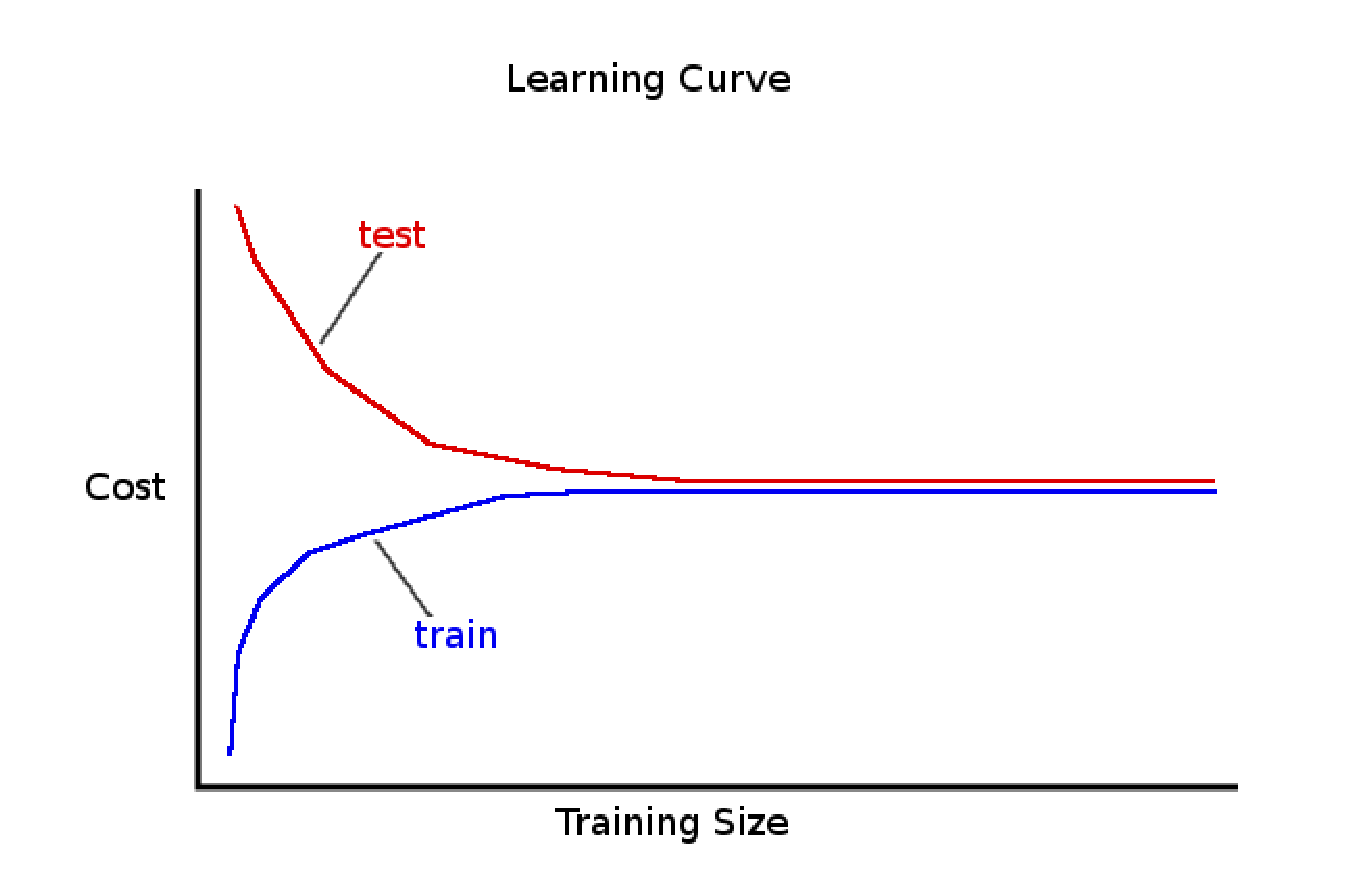
\includegraphics[height=3in]{04ANNlearncurve/LCHighBias.eps}
\end{center}
\caption{ภาพคร่าวๆของ\textit{เส้นโค้งเรียนรู้}ในกรณีที่โมเดลมีไบอัสสูง (High Bias). 
เมื่อจำนวนของจุดข้อมูลฝึกมากขึ้น ค่าผิดพลาดของชุดฝึกและค่าผิดพลาดของชุดทดสอบมีค่าใกล้เคียงกัน.}
\label{fig: more ann learning curve high bias}
\end{figure}

%
\begin{figure}
\begin{center}
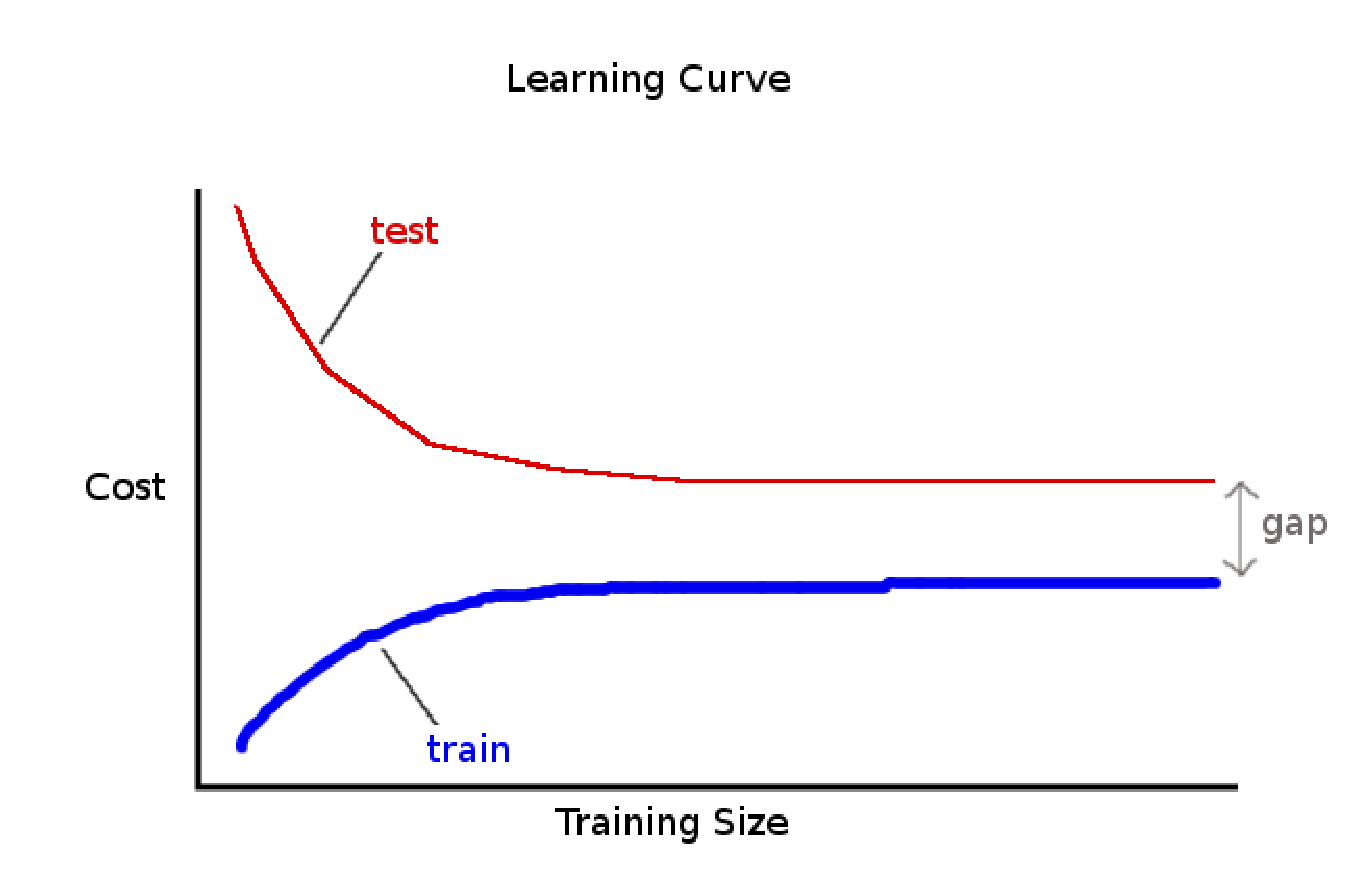
\includegraphics[height=3in]{04ANNlearncurve/LCHighVariance.eps}
\end{center}
\caption{ภาพคร่าวๆของ\textit{เส้นโค้งเรียนรู้}ในกรณีที่โมเดลมีความแปรผันสูง (High Variance). เมื่อจำนวนของจุดข้อมูลฝึกมากขึ้น ค่าผิดพลาดของชุดฝึกและค่าผิดพลาดของชุดทดสอบมีค่าห่างกัน}
\label{fig: more ann learning curve high variance}
\end{figure}

ทั้งรูป~\ref{fig: more ann learning curve high bias} และ~\ref{fig: more ann learning curve high variance} เป็นภาพวาดคร่าวๆ เพื่อให้เห็นภาพรวม.
ในความเป็นจริง \textit{เส้นโค้งเรียนรู้}ที่วาดอาจจะมีสัญญาณรบกวนมาก 
หรือแม้แต่\textit{สเกลของการวาดกราฟ}อาจทำให้ต้องใช้ความระมัดระวังใน\textit{การอ่านเส้นโค้งเรียนรู้}.
หัวข้อ~\ref{sec: ann more learning curve example} แสดงตัวอย่างของ\textit{เส้นโค้งเรียนรู้}
จากโจทย์การหาค่าถดถอยมิติเดียว. % ที่ได้อภิปรายในหัวข้อ~\ref{sec: simple example}.

\subsubsection{เส้นโค้งเรียนรู้สำหรับต้วอย่างการหาค่าถดถอยมิติเดียว}
\label{sec: ann more learning curve example}

จากตัวอย่างง่ายๆ (หัวข้อ~\ref{sec: simple example} และ \ref{sec: ann app code simple example}) หากทดลองวาด\textit{เส้นโค้งเรียนรู้}ของโมเดลโครงข่ายประสาทเทียมที่ใช้แค่ $1$ หน่วยซ่อน จะได้ผลดังรูป~\ref{fig: more ann learning curve high bias M1}.
%สำหรับ ค่าผิดพลาดของชุดทดสอบ, ที่จำนวนจุดข้อมูลฝึกน้อยๆ โมเดลไม่ได้ให้ เอาต์พุตที่ดีพอ สำหรับ ข้อมูลที่ไม่เคยเห็นมาก่อน, ค่าผิดพลาดของชุดทดสอบจึงเริ่มจากสูงมาก
%และ เมื่อมีข้อมูลฝึกมากขึ้น โมเดลก็สามารถปรับปรุง คุณสมบัติความทั่วไป ได้ดีขึ้น จึงทำให้ ค่าผิดพลาดของชุดทดสอบลดลง.
%แต่สำหรับ ค่าผิดพลาดของชุดฝึก,
%ที่จำนวนจุดข้อมูลฝึกน้อยๆ โมเดลสามารถให้เอาต์พุตผ่านจุดฝึกได้สมบูรณ์ ค่าผิดพลาดของชุดฝึก จึงเริ่มจาก $0$ แล้วเมื่อจุดฝึกเพิ่มขึ้น โมเดลไม่สามารถให้เอาต์พุตที่ผ่านจุดฝึกได้ทุกจุด ค่าผิดพลาดจึงเพิ่มขึ้น เมื่อจำนวนจุดฝึกเพิ่มขึ้น.
%และ ลู่เข้าหาค่าคงที่เมื่อ จำนวนจุดฝึกมากเพียงพอ สำหรับความยืดหยุ่นของโมเดล.
%ความยืดหยุ่นของโมเดลที่จำกัด ทำให้โมเดลไม่สามารถลดค่าผิดพลาดของชุดทดสอบลงได้อีก.
%และ ค่าผิดพลาดของทั้งชุดฝึก และ ชุดทดสอบ จึง มีค่าใกล้เคียงกัน เมื่อจำนวนข้อมูลฝึกมีมากๆ.
%แต่ความยืดหยุ่นของโมเดลจำกัด ค่าผิดพลาดนี้จึงลดลงถึงได้แค่ระดับหนึ่ง ถึงแม้ว่าจะมีจำนวนข้อมูลฝึกมากขึ้น

%
\begin{figure}
\begin{center}
\includegraphics[width=5.5in]{04ANNlearncurve/LCHiBiasM1.eps}
\end{center}
\caption{เส้นโค้งเรียนรู้ในกรณีไบอัสสูง. 
เส้นโค้งเรียนรู้ (ภาพซ้ายบนสุด) 
เส้นกราฟที่ใช้สัญญลักษณ์ `o' แทนค่าผิดพลาดของชุดฝึก
เส้นกราฟที่ใช้สัญญลักษณ์ `*' แทนค่าผิดพลาดของชุดทดสอบ.
ที่จำนวนจุดข้อมูลมากๆ (ปลายของเส้นโค้งเรียนรู้) ค่าผิดพลาดของชุดฝึกและค่าผิดพลาดของชุดทดสอบมีค่าใกล้เคียงกัน. 
อัตราส่วน $\frac{E_{\mathrm{test}}}{E_{\mathrm{train}}}$ (ภาพขวาบนสุด) มีค่าราวๆ $1.1$ ที่ปลายของเส้นโค้งเรียนรู้.
ภาพอื่นๆแสดงเอาต์พุตที่ได้จากโมเดล (เส้นกราฟ) เมื่อฝึกด้วย $1$, $5$, $10$, $15$, $20$, และ $50$ จุดข้อมูล ตามระบุที่ชื่อภาพ.
จุดข้อมูลที่ใช้ฝึกแสดงด้วยสัญญลักษณ์ `o' และจุดข้อมูลที่ใช้ทดสอบแสดงด้วยสัญญลักษณ์ `x'
}
\label{fig: more ann learning curve high bias M1}
\end{figure}

ภาพของเอาต์พุตหลังจากฝึกด้วยจำนวนจุดข้อมูลต่างๆ ในรูป~\ref{fig: more ann learning curve high bias M1} แสดงให้เห็นว่า การใช้โครงข่ายประสาทเทียม $1$ หน่วยซ่อนนั้น ทำให้โมเดลไม่มีความยืดหยุ่นเพียงพอ.
กรณีนี้คือไบอัสสูง และเส้นโค้งเรียนรู้ในภาพซ้ายบนสุดก็แสดงการลู่เข้าของค่าผิดพลาดจากทั้งชุดฝึกและชุดทดสอบ.
สังเกตุว่า ค่าผิดพลาดทั้งสองลู่เข้าสู่ค่าประมาณ $20$.
และ เพื่อตรวจสอบดูว่าค่าทั้งสองลู่เข้าใกล้กันมากขนาดไหน 
\textit{ภาพขวาบนสุด}แสดง\textit{อัตราส่วนระหว่างค่าผิดพลาดชุดทดสอบและชุดฝึกหัด}.
ที่จำนวนข้อมูลฝึกมากๆ (ปลายเส้นโค้งเรียนรู้) อัตราส่วนนี้ลู่เข้าหาค่าประมาณ $1.1$.
อัตราส่วนที่มีค่าใกล้ $1$ นี้บ่งบอกว่าค่าผิดพลาดทั้งสองมีค่าใกล้กันมาก.

เปรียบเทียบผลข้างต้นกับ\textit{กรณีที่โมเดลมีความแปรผันสูง}
ความแปรผันสูงเกี่ยวพันกับการที่โมเดลมีความยืดหยุ่นมากเกินไป.
จากตัวอย่างเดียวกัน เมื่อใช้โครงข่ายประสาทเทียมที่มี $2000$ หน่วยซ่อน เส้นโค้งเรียนรู้ที่ได้แสดงดังรูป~\ref{fig: more ann learning curve high variance M2000}.

%
\begin{figure}
\begin{center}
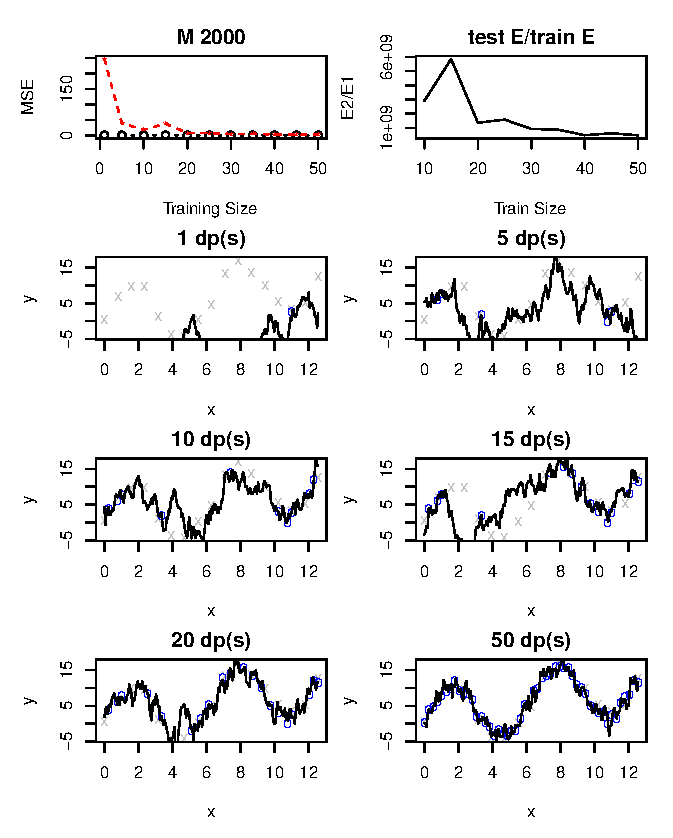
\includegraphics[width=5.5in]{04ANNlearncurve/LCHiVarianceM2000.eps}
\end{center}
\caption{เส้นโค้งเรียนรู้ในกรณีความแปรผันสูง.
เส้นโค้งเรียนรู้ (ภาพซ้ายบนสุด) 
เส้นกราฟที่ใช้สัญญลักษณ์ `o' แทนค่าผิดพลาดของชุดฝึก
เส้นกราฟที่ใช้สัญญลักษณ์ `*' แทนค่าผิดพลาดของชุดทดสอบ. 
ที่จำนวนจุดข้อมูลมากๆ (ปลายของเส้นโค้งเรียนรู้) ค่าผิดพลาดของชุดฝึกและค่าผิดพลาดของชุดทดสอบมีค่าต่างกันมาก.
กราฟในภาพซ้ายบนสุดอาจมองเห็นความต่างไม่ชัดเจน แต่อัตราส่วน $\frac{E_{\mathrm{test}}}{E_{\mathrm{train}}}$ (ภาพขวาบนสุด) โดยเฉพาะ%ที่มีค่าเกือบๆ $10^9$ 
ที่ปลายของเส้นโค้งเรียนรู้ ช่วยเน้นถึงความแตกต่างนี้ 
(สังเกตุสเกลของค่าอัตราส่วนที่แกนตั้ง.
ค่า \texttt{1e+09} คือ $10^9$)
ภาพอื่นๆแสดงเอาต์พุตที่ได้จากโมเดล (เส้นกราฟ) เมื่อฝึกด้วย $1$, $5$, $10$, $15$, $20$, และ $50$ จุดข้อมูล ตามระบุที่ชื่อภาพ
จุดข้อมูลที่ใช้ฝึกแสดงด้วยสัญญลักษณ์ `o' 
และจุดข้อมูลใช้ทดสอบแสดงด้วยสัญญลักษณ์ `x'}
\label{fig: more ann learning curve high variance M2000}
\end{figure}

ภาพของเอาต์พุตหลังจากผ่านการฝึกด้วยจำนวนจุดข้อมูลต่างๆ ที่แสดงในรูป~\ref{fig: more ann learning curve high variance M2000} ยืนยันว่า การใช้โครงข่ายประสาทเทียมสองชั้นขนาด $2000$ หน่วยซ่อนนั้น 
ทำให้โมเดลมีความยืดหยุ่นมากเกินไป มากจนโมเดลไปปรับเข้ากับสัญญาณรบกวนในข้อมูลฝึกได้.
กรณีนี้แสดงถึง\textit{ความแปรผันสูง}อย่างชัดเจน.

ภาพซ้ายบนสุดของรูป~\ref{fig: more ann learning curve high variance M2000} แสดงเส้นโค้งเรียนรู้ ที่ค่าผิดพลาดทั้งสองลู่เข้าแล้ว.
แต่เนื่องจากสเกลของภาพ จึงทำให้บอกได้ยากว่า ค่าผิดพลาดที่ลู่เข้าทั้งสองนั้นใกล้เคียงหรือห่างกันมากขนาดไหน.
\textit{อัตราส่วนค่าผิดพลาด}ที่แสดงในภาพขวาบนสุดช่วยบอกความต่างระหว่างค่าผิดพลาดทั้งสอง.
สังเกตุค่าอัตราส่วนนี้ที่ปลายของกราฟ ซึ่งมีค่ามาก (ราวๆ $10^9$ เท่า). % อัตราส่วนนี้อยู่ที่ราวๆ $10^9$ เท่า.
นั่นคือ ค่าผิดพลาดทั้งสองต่างกันมาก บ่งบอกถึงกรณีความแปรผันสูงอย่างชัดเจน.
%
%รูป~\ref{fig: ANN more learning curves example} แสดงเส้นโค้งเรียนรู้ ของโครงข่ายประสาทเทียมที่จำนวนหน่วยซ่อนต่างๆ.

ตัวอย่างในหัวข้อ~\ref{sec: simple example} ใช้โครงข่ายประสาทเทียม $20$ หน่วยซ่อน.
หากลองนำเส้นโค้งเรียนรู้มาวาดดังแสดงในรูป~\ref{fig: ANN more learning curves example M20}
จะเห็นว่า ที่ปลายเส้นโค้งเรียนรู้ ค่าผิดพลาดของชุดฝึกค่อนข้างห่างจากค่าผิดพลาดของชุดทดสอบ (ค่าอัตราส่วนความผิดพลาดประมาณกว่า $5$ เท่า ภาพที่ 3 จากซ้าย)
ดังนั้นโครงข่ายประสาทเทียมขนาด $20$ หน่วยซ่อนกับปัญหาตัวอย่างในหัวข้อ~\ref{sec: simple example} จะเข้ากรณีของความแปรผันสูง.
และภาพขวาสุดยังแสดงให้เห็นอย่างชัดเจนว่า เอาต์พุตจากโครงข่ายได้ปรับตัวไปเข้ากับสัญญาณรบกวนของข้อมูลฝึกบ้างแล้ว.

%
\begin{figure}
\begin{center}
\includegraphics[height=1.5in]{04ANNlearncurve/LCM20.eps}
\end{center}
\caption{เส้นโค้งเรียนรู้.
ภาพซ้ายสุดแสดงเส้นโค้งเรียนรู้
เส้นทึบสัญญลักษณ์ `o' แทนค่าผิดพลาดของชุดฝึก
เส้นประสัญญลักษณ์ `*' แทนค่าผิดพลาดของชุดทดสอบ.
ภาพที่สองจากซ้ายแสดงเส้นโค้งเรียนรู้ด้วยสเกลขยาย 
เพื่อตรวจสอบความห่างของค่าผิดพลาดสองชุดได้ชัดเจนขึ้น.
ภาพที่สามจากซ้ายแสดงค่าอัตราส่วนความผิดพลาด.
ภาพขวาสุดแสดงเอาต์พุตของโครงข่ายหลังจากฝึกด้วยจำนวนจุดข้อมูลฝึกทั้งหมด
เส้นทึบแทนค่าเอาต์พุตจากโครงข่ายประสาทเทียม
สัญญลักษณ์ `o' แทนจุดข้อมูลฝึก
สัญญลักษณ์ `x' แทนจุดข้อมูลทดสอบ.}
\label{fig: ANN more learning curves example M20}
\end{figure}

ตัวอย่างข้างต้นแสดงปัญหาการหาค่าถดถอย ที่อินพุตมีมิติเดียว.
อินพุตมิติเดียวช่วยให้เรามองเห็น กรณีทั้งไบอัสสูงและความแปรผันสูงได้ชัดเจนขึ้น.
ปัญหาที่อาจเจอในทางปฏิบัติ
อาจไม่ได้มีธรรมชาติที่ช่วยให้สามารถวาดเอาต์พุตของโมเดลมาดูเทียบกับจุดข้อมูลฝึกหัดและจุดข้อมูลทดสอบได้ง่ายเช่นนี้.
ดังนั้นจึงใช้\textit{เส้นโค้งเรียนรู้}และ\textit{ความห่างที่ค่าผิดพลาดของชุดฝึกและชุดทดสอบ} เพื่อบ่งชี้กรณีไบอัสสูง หรือความแปรผันสูง สำหรับการวิเคราะห์การทำโมเดล.
หัวข้อ~\ref{sec: ann more suggested options} อภิปรายทางเลือกที่แนะนำ 
เพื่อปรับปรุงคุณภาพโมเดล%โครงการประยุกต์ใช้การเรียนรู้ของเครื่อง 
ตามกรณีไบอัสสูงหรือความแปรผันสูง.

\subsection{ทางเลือกที่แนะนำ}
\label{sec: ann more suggested options}

หลังจากพอรู้แล้วว่า \textit{สถานะการณ์ของโมเดลที่ใช้อยู่}เข้ากรณีไบอัสสูงหรือกรณีความแปรผันสูง
ก็สามารถพิจารณาทางเลือกได้ ดังนี้
\begin{itemize}
\item \emph{เก็บข้อมูลมาเพิ่มสำหรับการฝึก.} % (collect more training examples),
การเพิ่มจำนวนข้อมูลในการฝึก จะช่วยในกรณีความแปรผันสูง
\item \emph{เลือกเฉพาะบางมิติของข้อมูลมาเป็นอินพุต.} % (select smaller sets of features),
การเลือกเฉพาะบางมิติของข้อมูลมาเป็นอินพุต (ลดมิติของอินพุตลง) ก็จะช่วยในกรณีความแปรผันสูง
\item \emph{เพิ่มลักษณะที่สำคัญใหม่เข้าไปในอินพุต.} % (get additional features),
การเพิ่มลักษณะที่สำคัญใหม่เข้าไปในอินพุต (เพิ่มมิติของอินพุตขึ้น) โดยทั่วไปแล้ว จะช่วยในกรณีไบอัสสูง
\item \emph{เพิ่มความซับซ้อนของโมเดลขึ้น.} % (try increase model's complexity), 
การเพิ่มความซับซ้อนของโมเดล เช่น การเพิ่มจำนวนหน่วยซ่อน จะช่วยในกรณีไบอัสสูง
\item \emph{ลดความซับซ้อนของโมเดลลง.} % (try decrease model's complexity),
การลดความซับซ้อนของโมเดล เช่น การลดจำนวนหน่วยซ่อน การใช้เรกูลาไรเซชั่น หรือ การทำการหยุดก่อนกำหนด จะช่วยในกรณีความแปรผันสูง.
\end{itemize}

ตาราง~\ref{tbl: ann tips options by bias variance} 
สรุปทางเลือกที่แนะนำสำหรับกรณีไบอัสสูงและกรณีความแปรผันสูง.
สุดท้ายหากลองวิธีทั่วๆไปดังนี้แล้ว ผลยังไม่ดีขึ้น หรือดีขึ้นแล้วแต่อยากให้ดีขึ้นอีก
ผู้ทำโมเดลอาจจะลองวิเคราะห์ตรวจสอบผลที่อัลกอริทึ่มทำผิด ดูว่าผิดลักษณะไหน อย่างไร.
เผื่อว่า ผู้ทำโมเดลอาจจะพบคุณสมบัติเฉพาะบางอย่างที่ผลมักจะผิด เช่น หากเป็นการจำแนกตัวเลขจากภาพ (ตัวอย่างในหัวข้อ~\ref{sec: ann app multiclass code}) อัลกอริทึ่มอาจจะจำแนกเลข 2 เป็นเลข 4 บ่อยๆ ซึ่งเมื่อผู้ทำโมเดลดูภาพของเลขที่จำแนกผิด ก็อาจพบว่า มีรูปแบบการเขียนเลข 2 แบบหนึ่ง ที่มักจะจำแนกผิด.
หากผู้ทำโมเดลพบรูปแบบเฉพาะนั้น ผู้ทำโมเดลก็อาจเพิ่มการจัดการเฉพาะสำหรับรูปแบบที่สันสนบ่อยๆนั้นได้ เป็นต้น.

%* Start w/ a simple algorithm that you can implement quickly (1 day). Implement it and test it on your cross validation data.
%* Plot learning curves to decide if more data, more featue, etc. are likely to help.
%* Do error analysis: manually examine the examples that your algorithm made errors on. See if you spot any systematic trend in what type of examples it is makig errors on.

\begin{table}[hbtp]
{\footnotesize %scriptsize
\caption{สรุปทางเลือกที่แนะนำในกรณีไบอัสสูงและความแปรผันสูง.}
\label{tbl: ann tips options by bias variance}
\begin{center}
\begin{tabular}{|l|c|c|}
\hline 
       & \multicolumn{2}{|c|}{กรณี} \\
       \cline{2-3}
ทางเลือก & ไบอัสสูง & ความแปรผันสูง \\
\hline
เพิ่มรอบฝึก            & แนะนำ      &   \\
เพิ่มจำนวนหน่วยย่อย     & แนะนำ      &   \\
ทำเรกูลาไรเซชั่น        &           & แนะนำ \\
ทำการหยุดก่อนกำหนด    &           & แนะนำ \\
ลดมิติของอินพุตลง       &           & แนะนำ \\
เพิ่มมิติของอินพุตขึ้น      & แนะนำ      &  \\
เพิ่มจำนวนจุดข้อมูลฝึก     &             & แนะนำ \\
%
\hline
\end{tabular} 
\end{center}
}%end \small
\end{table}



\section{แบบฝึกหัด}
\label{section: ANN more exercises}

\paragraph{1.} จงหาฟังชั่นค่าอนุพันธ์ของสมการ~\ref{eq: ann more gdm example} และ นำฟังชั่นค่าอนุพันธ์ที่ได้มาเขียนโปรแกรม และวาดรูปเลียบแบบรูป~\ref{fig: more ann gdm}.
รูป~\ref{fig: more ann gdm} ใช้ค่าเริ่มต้น $[x_1, x_2]^{(0)} = [2.5, 3]$ ค่าขนาดก้าว (ทั้งวิธีลงเกรเดียนต์ และ วิธีลงเกรเดียนต์กับโมเมนตัม) $0.125$ และค่าอัตราโมเมนตัม $0.1$.
เปรียบเทียบคำตอบสุดท้ายที่ได้ จำนวนรอบฝึกที่ใช้ และเวลาที่ใช้ ของทั้งสามวิธี.

\paragraph{2.} จากข้อ 1 จงทดลองวิธีลงเกรเดียนต์กับโมเมนตัม ที่ค่าขนาดก้าวและอัตราโมเมนตัมต่างๆ.
สรุปผล และอภิปราย.

\paragraph{3.} จงนำ\textit{วิธีลงเกรเดียนต์กับโมเมนตัม}ไปใช้กับฝึกโครงข่ายประสาทเทียม.
\emph{คำใบ้.} $\mathbf{w}$ ในสมการ~\ref{eq: ann more gd momentum update weights} คือ ค่าน้ำหนัก.
ทดสอบการทำงานกับปัญหาการหาค่าถดถอย ปัญหาการจำแนกกลุ่มแบบสองกลุ่ม และปัญหาการจำแนกกลุ่มแบบหลายกลุ่ม.
เปรียบเทียบผลการฝึกกับการฝึกด้วยวิธีลงเกรเดียนต์ สรุปผล และอภิปราย.

\paragraph{4.} จงออกแบบการทดลอง และทดลองผลการทำงานของโครงข่ายประสาทเทียม เมื่อกำหนดค่าเริ่มต้นด้วยการสุ่มจากการแจกแจงแบบเอกรูป (uniform distribution) 
เปรียบเทียบกับการกำหนดค่าเริ่มต้นด้วย\textit{วิธีเหงี่ยน-วิดโดรว์}.
สรุปและอภิปรายผล.
\emph{หมายเหตุ} ให้ทดลองฝึกด้วยวิธีลงเกรเดียนต์ วิธีบีเอฟจีเอส และวิธีเอสซีจี 
และทดลองประยุกต์กับปัญหาหลากหลายแบบ เช่น การหาค่าถดถอย การจำแนกกลุ่ม และการจำแนกกลุ่มหลายกลุ่ม.

\paragraph{5.} จงออกแบบการทดลอง และทดลองผลการทำงานของโครงข่ายประสาทเทียม 
เมื่อใช้วิธีฝึกต่างๆ ได้แก่ วิธีลงเกรเดียนต์, วิธีบีเอฟจีเอส และวิธีเอสซีจี กับปัญหาหลากหลายแบบ 
เช่น การหาค่าถดถอย การจำแนกกลุ่ม และการจำแนกกลุ่มหลายกลุ่ม.
สรุปและอภิปรายผล.

\paragraph{6.} จากตัวอย่างในหัวข้อ~\ref{sec: simple example} 
จงสร้างเส้นโค้งเรียนรู้ของโครงข่ายประสาทเทียมขนาด $20$ หน่วยย่อย 
เพื่อเปรียบเทียบกับรูป~\ref{fig: ANN more learning curves example M20}.
อภิปรายผล.
\emph{หมายเหตุ} รูป~\ref{fig: ANN more learning curves example M20} ได้จากการใช้ โครงข่ายประสาทเทียมขนาด $20$ หน่วยซ่อน ที่ฝึกด้วยวิธีเอสซีจี แบบไม่ทำการหยุดก่อนกำหนด และรอบการฝึกสูงสุดคือ $500$ รอบ และจะจบก่อนถึงรอบฝึกสูงสุดได้ เมื่อค่าฟังชั่นจุดประสงค์เปลี่ยนแปลงน้อยกว่า $10^{-8}$ หรือ ค่าเฉลี่ยของเกรเดียนต์ยกกำลังสองน้อยกว่า $10^{-12}$.

\paragraph{7.} จากแบบฝึกหัดข้อ 6 จงทดลองปรับปรุงคุณภาพการทำนายของโครงข่ายประสาทเทียม โดยใช้ผลจากเส้นโค้งเรียนรู้ประกอบ. 
สรุปสิ่งที่ได้ทดลองทำ อภิปรายสิ่งที่ได้เรียนรู้ ชี้แจงเหตุผลที่รองรับ และวิเคราะห์ผลจากการทดลองหลังการปรับปรุง.

\paragraph{8.} จงใช้เส้นโค้งเรียนรู้เพื่อวิเคราะห์การทำงานของโครงข่ายกับตัวอย่างการหาค่าถดถอย ในหัวข้อ~\ref{sec: regression example code}.
จงทดลองทำการปรับปรุง สรุปและอภิปรายการทดลองและผล.

\paragraph{9.} จงใช้เส้นโค้งเรียนรู้เพื่อวิเคราะห์การทำงานของโครงข่ายกับตัวอย่างการจำแนกกลุ่ม ในหัวข้อ~\ref{sec: ann biclass example}.
จงทดลองทำการปรับปรุง สรุปและอภิปรายการทดลองและผล.

\paragraph{10.} จงใช้เส้นโค้งเรียนรู้เพื่อวิเคราะห์การทำงานของโครงข่ายกับตัวอย่างการจำแนกกลุ่มแบบหลายกลุ่ม ในหัวข้อ~\ref{sec: ann app multiclass code}.
จงทดลองทำการปรับปรุง สรุป และอภิปรายการทดลองและผล.